%%%%%%%%%%%%2019.3.12第三周Mon%%%%%%%%%%%%%%%%%%%%%%%
%%%%%%%%%%%%%%%%下周一,邱宇代课%%&%%%%%%%%%%%%%%%%%%
%%%%%%%%%%%%%%%%下周二,随堂考试%%%%%%%%%%%%%%%%%%%%%

%\textbf{Coalgebra and homotopy associativity}



\chapter{形变量子化}

%%%%%%%%%%2019.3.18第四周 周一%%%%%%%%%%%%%%%%%%%%%%%
%%%%%%%%%%%%%%%%李思出差,别人代课%%%%%%%%%%%%%%%%%%%
本章开始,正式搞一些事情。
经典力学与量子力学的框架众所周知,大致如下:

\index{phase space\kong 相空间}
\index{symplectic manifold\kong 辛流形}
\index{observable\kong 观测量}
\index{Hamiltonian\kong 哈密顿量}

$$
  \begin{tabular}{|c|c|c|}
    \hline
             &经典力学 &量子力学\\
    \hline
    相空间   &辛流形$(X,\omg)$   &希尔伯特空间$\mcalH$\\
    观测量   &光滑函数           &厄密特算子  \\
    演化方程 &$\frac{\td f}{\td t}=\{H,f\}$
    &$\frac{\td A_t}{\td t}=\frac{i}{\hbar}[\hat{H},A_t]$\\
    \hline
  \end{tabular}
$$

我们将利用结合代数的Hochschild(上)同调,以及$A_{\infty}$方法,
来证明Kontsevich的Formality theorem.

{\color{red}(待完善)}

%\textbf{Poisson structure and quantization}

%Motiration
%Classical Mechanics
%Phase space$(X,\omg)\rightsquigarrow$ Sympletic mfd
%observables: $C^{\infty}(X)$: smooth function
%Poisson bracket:
%$C^{\infty}(X)\ten X^{\infty}(X)\to C^{\infty}(X)$
%Dynamics - Hamiltionian function $H\in C^{\infty}(X)$
%s.t. $\frac{\td f}{\td t}=\{H,f\}$.

%Quantum Picture:
%Hilbert space
%$$\frac{\td A_t}{\td t}=\frac{i}{\hbar}[\hat{H},A_t]$$
%Associative algebra.
%$A_{\infty}$-method and Hochcshild homology
%\textbf{Goal: Formality thm(Kontsevich)}
%Now, let us begin...
%\vs

\section{泊松几何与辛几何}
%\textbf{Poisson bracket}

本节简要回顾一下泊松几何。

\begin{definition}(泊松括号)
\index{Poisson bracket\kong 泊松括号}
%let $X$ be a smooth manifold, a Poisson bracket
%on $C^{\infty}(X)$ is  a $\bbR$-linear
%$$\{,\}:C^{\infty}(X)\times C^{\infty}(X)\to C^{\infty}(X)$$
%sarisfies
%skew symmetry
%Leibnitz rule
%Jacobi identity

设$X$为光滑流形,$\{,\}:C^{\infty}(X)\times C^{\infty}(X)\to C^{\infty}(X)$
为$\bbR$-双线性映射。称$\{,\}$为$X$上的\textbf{泊松括号}(Poisson bracket),
如果$\{,\}$满足:
对任意$f,g,h\in C^{\infty}(X)$,成立

(1)反对称性:$$\{f,g\}=-\{g,f\}$$

(2)Jacobi恒等式:
$$\{f,\{g,h\}\}+\{g,\{h,f\}\}+\{h,\{f,g\}\}=0$$

(3)Leibnitz法则:
$$\{f,gh\}=\{f,g\}h+g\{f,h\}$$
\end{definition}


泊松括号的定义的(1)(2)表明$(C^{\infty}(X),\{,\})$为李代数,
而(3)表明对任意$f\in C^{\infty}(X)$,映射
\begin{eqnarray*}
X_f:C^{\infty}(X)&\to& C^{\infty}(X)\\
g &\mapsto& \{f,g\}
\end{eqnarray*}
为导子,从而$X_f$为$X$上的光滑切向量场,
在局部坐标下形如$X_f=X_f^i\pp{u^i}$.于是有
$$\{f,g\}=X_f^i\pfrac{g}{u^i}$$
但又注意到$\{f,g\}=-\{g,f\}$以及切向量场$X_g$,
从而易知泊松括号$\{,\}$在局部坐标$(u^i)$下的表达式必形如
$$\{f,g\}=P^{ij}\pfrac{f}{u^i}\pfrac{g}{u^j}$$
并且容易验证:
\begin{lemma}设$\{,\}$为光滑流形$X$上的泊松括号,
并且在局部坐标$(u^i)$下的表达式为
$$\{f,g\}=P^{ij}\pfrac{f}{u^i}\pfrac{g}{u^j}$$
那么对任意指标$i,j,k$,成立
$$P^{ij}=-P^{ji}$$
$$P^{is}\pfrac{P^{jk}}{u^s}+
P^{js}\pfrac{P^{ki}}{u^s}+
P^{ks}\pfrac{P^{ij}}{u^s}=0$$
\end{lemma}

\begin{proof}
容易验证$P^{ij}=-P^{ji}$等价于泊松括号的反对称性$\{f,g\}=-\{g,f\}$,
这是因为对任意光滑函数$f,g$,局部上有
$$P^{ij}\pfrac{f}{u^i}\pfrac{g}{u^j}=\{f,g\}=-\{g,f\}
=-P^{ij}\pfrac{g}{u^i}\pfrac{f}{u^j}=
-P^{ji}\pfrac{f}{u^i}\pfrac{g}{u^j}$$
从而$(P^{ij}+P^{ji})\pfrac{f}{u^i}\pfrac{g}{u^j}=0$,
因此由$f,g$的任意性,有$P^{ij}=-P^{ji}$.\vs

再看第二个式子。事实上它等价于泊松括号的雅可比恒等式。
对任意$f,g,h\in C^{\infty}(X)$,局部坐标下有
\begin{eqnarray*}
     \{f,\{g,h\}\}
&=&
     \{f,P^{ij}\pfrac{g}{u^i}\pfrac{h}{u^j}\}\\
&=&
     P^{kl}\pfrac{f}{u^k}
     \pfrac{P^{ij}}{u^l}
     \pfrac{g}{u^i}
     \pfrac{h}{u^j}
    +P^{ij}P^{kl}\pfrac{f}{u^k}
     \left(
       \pmfrac{g}{u^i}{u^l}\pfrac{h}{u^j}
      +\pmfrac{h}{u^j}{u^l}\pfrac{g}{u^i}
     \right)
\end{eqnarray*}
将$f,g,h$轮换再相加,适当更改求和指标,合并整理得
\begin{eqnarray*}
& &
     \{f,\{g,h\}\}+\{g,\{h,f\}\}+\{h,\{f,g\}\}\\
&=&
     \pfrac{f}{u^i}
     \pfrac{g}{u^j}
     \pfrac{h}{u^k}
     \left(
       P^{is}\pfrac{P^{jk}}{u^s}
      +P^{js}\pfrac{P^{ki}}{u^s}
      +P^{ks}\pfrac{P^{ij}}{u^s}
     \right)
    +P^{kl}(P^{ij}+P^{ji})
     \pfrac{f}{u^k}
     \pmfrac{g}{u^i}{u^l}
     \pfrac{h}{u^j}\\
& &
    +P^{kl}(P^{ij}+P^{ji})
     \pfrac{g}{u^k}
     \pmfrac{h}{u^i}{u^l}
     \pfrac{f}{u^j}
    +P^{kl}(P^{ij}+P^{ji})
     \pfrac{h}{u^k}
     \pmfrac{f}{u^i}{u^l}
     \pfrac{g}{u^j}
\end{eqnarray*}
注意到$P^{ij}=-P^{ji}$,以及$f,g,h$的任意性,从而有
$$
 P^{is}\pfrac{P^{jk}}{u^s}
+P^{js}\pfrac{P^{ki}}{u^s}
+P^{ks}\pfrac{P^{ij}}{u^s}
=0
$$
得证。
\end{proof}

我们可以使用张量的语言来描述泊松括号结构:

\begin{definition}(泊松张量)
对于光滑流形$X$,以及$P\in\PV^2_X$为$2$-切向量场,
在局部坐标下表达式为
$$P=P^{ij}\pp{u^i}\wedge\pp{u^j}$$
其中$P^{ij}=-P^{ji}$.称$P$为\textbf{泊松张量}(Poisson tensor),
\index{Poisson tensor\kong 泊松张量}
如果$P$在局部坐标下满足如下雅可比恒等式:
$$
 P^{is}\pfrac{P^{jk}}{u^s}
+P^{js}\pfrac{P^{ki}}{u^s}
+P^{ks}\pfrac{P^{ij}}{u^s}
=0
$$
\end{definition}
容易看出泊松括号与泊松张量的一一对应关系:
对于泊松括号$\{,\}$,若局部上有
$\{f,g\}=P^{ij}\pfrac{f}{u^i}\pfrac{g}{u^j}$,
则考虑泊松张量
$$P:=\frac{1}{2}P^{ij}\pp{u^i}\wedge\pp{u^j}$$
反过来,由泊松张量也能得到泊松括号。并且容易知道
$$\{f,g\}=\langle P,\td f\wedge\td g\rangle$$

%Poisson tensor:
%$P\in\Gamma(X,\wedgeform{2}TX)=\PV_X^2$ s.t.
%$$\{f,g\}=\langle P, \td f\wedge \td g\rangle$$
%$$=P^{ij}(\p_i f\p_jg-\p_ig\p_jf)$$

%Check: Jacobi identity $\iff[P,P]=0$, where
%$[,]$ is Schouten-Nijenhuis bracket.

事实上泊松张量的雅可比恒等式可以用Schouten-Nijenhuis括号等价刻画:

\begin{prop}对于光滑流形$X$,以及$P\in\PV^2_X$,
则$P$为泊松张量当且仅当
$$[P,P]=0$$
其中$[,]$为Schouten-Nijenhuis括号
(见定义\ref{Schouten-Nijenhuis定义-def})。
\end{prop}

\begin{proof}
局部坐标下验证。取局部坐标$(u^i)$,
令$P=P^{ij}\pp{u^i}\wedge\pp{u^j}$,则有
\begin{eqnarray*}
     [P,P]
&=&
     \big[(P^{ij}\pp{u^i})\wedge\pp{u^j},
     (P^{kl}\pp{u^k})\wedge\pp{u^l}\big]\\
&=&
     [P^{ij}\pp{u^i},P^{kl}\pp{u^k}]\wedge\pp{u^j}\wedge\pp{u^l}
    -[P^{ij}\pp{u^i},\pp{u^l}]\wedge\pp{u^j}\wedge P^{kl}\pp{u^k}\\
& &
    -[\pp{u^j},P^{kl}\pp{u^k}]\wedge P^{ij}\pp{u^i}\wedge\pp{u^l}
    +[\pp{u^j},\pp{u^l}]\wedge P^{ij}\pp{u^i}\wedge P^{kl}\pp{u^k}
\end{eqnarray*}
上式右端共有四项,首先注意最后一项
$$[\pp{u^j},\pp{u^l}]\wedge P^{ij}\pp{u^i}\wedge P^{kl}\pp{u^k}
=P^{ij}P^{kl}\delta_{jl}\pp{u^j}\wedge\pp{u^i}\wedge\pp{u^k}
=\sum_{j=1}^nP^{ij}P^{kj}
 \pp{u^j}\wedge\pp{u^i}\wedge\pp{u^k}=0$$
最后一个等号是因为指标$i,k$的(反)对称性;
从而暴力展开,注意利用$P^{ij}=-P^{ji}$以及适当更改求和指标,有
\begin{eqnarray*}
     [P,P]
&=&
     [P^{ij}\pp{u^i},P^{kl}\pp{u^k}]\wedge\pp{u^j}\wedge\pp{u^l}\\
& &
    -[P^{ij}\pp{u^i},\pp{u^l}]\wedge\pp{u^j}\wedge P^{kl}\pp{u^k}
    -[\pp{u^j},P^{kl}\pp{u^k}]\wedge P^{ij}\pp{u^i}\wedge\pp{u^l}\\
&=&
     P^{ij}\pfrac{P^{kl}}{u^i}
     \pp{u^k}\wedge\pp{u^j}\wedge\pp{u^l}
    -P^{kl}\pfrac{P^{ij}}{u^k}
     \pp{u^i}\wedge\pp{u^j}\wedge\pp{u^l}\\
& &
    +P^{kl}\pfrac{P^{ij}}{u^l}
     \pp{u^i}\wedge\pp{u^j}\wedge\pp{u^k}
    -P^{ij}\pfrac{P^{kl}}{u^j}
     \pp{u^k}\wedge\pp{u^i}\wedge\pp{u^l}\\
&=&
     \left(
       -P^{sj}\pfrac{P^{ki}}{u^s}
       -P^{sk}\pfrac{P^{ij}}{u^s}
       +P^{ks}\pfrac{P^{ij}}{u^s}
       -P^{js}\pfrac{P^{ik}}{u^s}
     \right)
     \pp{u^i}\wedge\pp{u^j}\wedge\pp{u^k}\\
&=&
     -4P^{sj}\pfrac{P^{ki}}{u^s}
     \pp{u^i}\wedge\pp{u^j}\wedge\pp{u^k}\\
&=&
     -8\sum_{i<j<k}
       \left(
          P^{sj}\pfrac{P^{ki}}{u^s}
         +P^{sk}\pfrac{P^{ij}}{u^s}
         +P^{si}\pfrac{P^{jk}}{u^s}
       \right)
     \pp{u^i}\wedge\pp{u^j}\wedge\pp{u^k}
\end{eqnarray*}
可见$[P,P]=0$当且仅当雅可比恒等式成立,证毕。
\end{proof}

于是我们自然地引入泊松流形的概念:

\begin{definition}(泊松流形)
\index{Poisson manifold\kong 泊松流形}

\textbf{泊松流形}(Poisson manifold)
是指二元组$(X,P)$,其中$X$为光滑流形,
$P\in\PV^2_X$满足$[P,P]=0$.
%A Poisson manifold is a pair $(X,P)$ such that
%$[P,P]=0$ for some $P\in\PV_X^2$.
\end{definition}
众所周知,这是经典力学的几何模型。
%(geometry of classical mechanics)
接下来看一些泊松流形的例子:

\begin{Example}(由辛结构诱导的泊松结构)
%if $(X,\omg)$ is a sympletic manifold,

设$(X,\omg)$为辛流形,其中辛形式
$$\omg=\frac{1}{2}\omg_{ij}\td x^i\wedge\td x^{j}$$
满足$\td\omg=0$,并且使得系数矩阵
$(\omg_{ij})_{1\leq i,j\leq n}$在$X$上处处可逆、反对称。
那么辛结构$\omg$自然诱导泊松结构
%such that $\omg$ is non-degenerated ,$\omg_{ij}=-\omg_{ji}$,
%then
$$\omg^{-1}:=\frac{1}{2}\omg^{ij}\p_i\wedge\p_j$$
其中矩阵$(\omg^{ij}):=(\omg_{ij})^{-1}$.
%is a Poisson bracket.where $(\omg^{ij}):=(\omg_{ij})^{-1}$
\end{Example}

\begin{proof}
我们只需验证雅可比恒等式
$$
  \omg^{is}\pfrac{\omg^{jk}}{u^s}
 +\omg^{js}\pfrac{\omg^{ki}}{u^s}
 +\omg^{ks}\pfrac{\omg^{ij}}{u^s}
=0
$$

一方面注意到逆矩阵求导公式
$\pfrac{\omg^{-1}}{u^s}=
-\omg^{-1}\pfrac{\omg}{u^s}\omg^{-1}$,从而有
$$\omg^{is}\pfrac{\omg^{jk}}{u^s}=-
\omg^{is}\omg^{jm}\omg^{nk}\pfrac{\omg_{mn}}{u^s}$$
对$i,j,k$轮换求和,有
$$
  \omg^{is}\pfrac{\omg^{jk}}{u^s}
 +\omg^{js}\pfrac{\omg^{ki}}{u^s}
 +\omg^{ks}\pfrac{\omg^{ij}}{u^s}
=
  \omg^{is}\omg^{jm}\omg^{kn}
  \left(
    \pfrac{\omg_{mn}}{u^s}
   +\pfrac{\omg_{ns}}{u^m}
   +\pfrac{\omg_{sm}}{u^n}
  \right)
$$

另一方面,由于$\td\omg=0$,从而有
\begin{eqnarray*}
     0
&=&
     \td(\omg_{ij}\td x^i\wedge\td x^j)\\
&=&
     \pfrac{\omg_{ij}}{u^k}\td x^i\wedge\td x^j\wedge\td x^k\\
&=&
     \sum_{i<j<k}
   2\left(
     \pfrac{\omg_{ij}}{u^k}
    +\pfrac{\omg_{jk}}{u^i}
    +\pfrac{\omg_{ki}}{u^j}
   \right)
   \td x^i\wedge\td x^j\wedge\td x^k
\end{eqnarray*}
因此有
$$\pfrac{\omg_{ij}}{u^k}
    +\pfrac{\omg_{jk}}{u^i}
    +\pfrac{\omg_{ki}}{u^j}=0$$

综上两方面,证毕。
\end{proof}
众所周知,这个例子来自经典力学。
事实上,此泊松结构有如下不依赖局部坐标的表达方式:
对任意$f\in C^{\infty}(X)$,存在唯一的切向量场$X_f$使得
$$\td f+i_{X_f}(\omg)=0$$
称此$X_f$为$f$的\textbf{哈密顿向量场}。
于是,对于任意的$f,g\in C^{\infty}(X)$,
辛结构$\omg$诱导的泊松括号满足
$$\{f,g\}=\omg(X_f,X_g)$$
以上是我们在经典力学中熟知的。下一个例子更“接近”经典力学:

\begin{Example}(光滑流形余切丛上的典范辛结构)

设$M$为$n$维光滑流形,$X:=T^*M$为$X$的余切丛,
则定义$X$上的\textbf{典范$1$-形式}$\theta\in\Omg^1_X$为:
$$\theta|_{(\bfx,\bfp)}(\bfv,\xi):=\langle \bfp,\bfv\rangle$$
其中$(\bfx,\bfp)\in X$,
$(\bfv,\xi)\in T_{(\bfx,\bfp)}(X)$,
以及$\bfv\in T_{\bfx}M$.
记$X$上的$2$-形式
$$\omg:=-\td\theta$$
称$\omg$为$T^*M$上的\textbf{典范辛形式}。
\end{Example}

考虑$X=T^*M$的局部坐标$(x^1,x^2,...,x^n;p_1,p_2,...,p_n)$,其中
$x^i$为$M$上的局部坐标。则容易知道典范$1$-形式
$\theta$与典范辛形式$\omg$在该局部坐标下的表达式分别为
$$\theta=\sum_{i=1}^np_i\td x^i$$
$$\omg=\sum_{i=1}^n\td x^i\wedge\td p_i$$

上述$\omg$给出了余切丛$T^*M$的辛流形结构,该辛结构诱导泊松结构,
于是我们可以谈论$X=T^*M$上的泊松括号。

\begin{rem}
记号承上,则存在典范的线性同态
\begin{eqnarray*}
\fai:\Gamma(M,TM)&\to& C^{\infty}(X)\\
\fai(\eta)|_{(\bfx,\bfp)}&=&\langle\bfp,\eta\rangle
\end{eqnarray*}
\label{切向量场视为余切丛上的光滑函数}
\end{rem}

即,通过“非常自然的方式”,将底流形$M$上的切向量场
视为余切丛$X=T^*M$上的光滑函数。该线性同态可以自然延拓到
切丛的对称张量丛的截面上:
$$\fai:\Gamma(M,\Sym(TM))\to C^{\infty}(X)$$
无非是“函数的相乘”而已。

\begin{prop}
设$M$为光滑流形,考虑$X=T^*M$上的典范辛结构,
$\fai:\Gamma(M,TM)\to C^{\infty}(X)$同上,
则对$M$的任意的切向量场$f,g$,成立
$$\fai([f,g])=-\{\fai(f),\fai(g)\}$$
其中左边“$[,]$”为$M$上的切向量场的李括号,
右边$\{,\}$为辛流形$X$上的泊松括号。
\end{prop}

\begin{proof}
局部坐标下验证。取$X$的局部坐标$(x^1,...,x^n;p_1,...,p_n)$,记
$$f=f^i\pp{x^i},\quad g=g^i\pp{x^i}$$
则容易知道
$$\fai(f)=f^i(\bfx)p_i,\quad \fai(g)=g^i(\bfx)p_i$$
注意$X$上的泊松张量
$$P=\pp{x^i}\wedge\pp{p_i}$$
因此有
\begin{eqnarray*}
     \{\fai(f),\fai(g)\}
&=&
     \Langle
       \pp{x^s}\wedge\pp{p_s}
     ,
       \td\fai(f)\wedge\td\fai(g)
     \Rangle\\
&=&
     \left(
       g^s\pfrac{f^i}{x^s}
      -f^s\pfrac{g^i}{x^s}
     \right)
     p_i
\end{eqnarray*}
而另一方面,
$$[f,g]=
\left(
  f^s\pfrac{g^i}{x^s}
 -g^s\pfrac{f^i}{x^s}
\right)\pp{x^i}
\quad\Longrightarrow\quad
\fai([f,g])=
\left(
  f^s\pfrac{g^i}{x^s}
 -g^s\pfrac{f^i}{x^s}
\right)p_i
$$
从而$\fai([f,g])=-\{\fai(f),\fai(g)\}$,得证。
\end{proof}

\section{形变量子化与Moyal星积}
%\textbf{Star product:}
我们开始讨论形变量子化。
{\color{red}(此处应该写几句introduction)}

\begin{definition}(星积)
%A star product $*$ on a Possion mfd $(X,P)$
%is a $\bbR[[\hbar]]$-linear map

对于泊松流形$(X,P)$,称$\bbR[\![\hbar]\!]$-双线性映射
\begin{eqnarray*}
C^{\infty}(X)\fps{\hbar}\times C^{\infty}(X)\fps{\hbar}
&\to& C^{\infty}(X)\fps{\hbar}\\
f\star g&\mapsto& \sum_{k\geq 0}C_k(f,g)\hbar^k
\end{eqnarray*}
为$(X,P)$上的\textbf{星积}(star product),
\index{star product\kong 星积}
%such that:
如果$\star$是结合的,并且对对任意$f,g\in C^{\infty}(X)$,以下成立:

%(1) 乘法$*$是结合的。 %is associative

(1) $\hbar\to 0$时退化为通常的函数乘法:
$$f\star g=fg\mod\hbar$$

(2) $*$的“一阶非交换性”由泊松括号给出:
$$f\star g-g\star f=\hbar\{f,g\}\mod\hbar^2$$
%$$\frac{1}{2}(f*g-g*f)=\hbar\{f,g\}\mod\hbar^2$$
%上一行被注掉的公式为笔记中的原始记载,我怀疑这个公式不对

(3) 对于每个$k\geq 0$,$C_k$为双微分算子:
$$C_k(f,g)=\sum_{\max{\{l,m\}}=k}
C_k^{i_1...i_l;j_1,...,j_m}(\p_{i_1}...\p_{i_l}f)
(\p_{j_1}...\p_{j_m}g)$$
其中系数$C_k^{i_1...i_l;j_1,...,j_m}\in C^{\infty}(X)$.
%, where $C_k^{...}$ is in $C^{\infty}(X)$.
%(bi-differential operator)
%\vs
%then, $(C^{\infty},*)$ is the \textbf{deformation quantization} on $(X,P)$.
\end{definition}

此时,也称$(C^{\infty}(X),\star)$为$(X,P)$的\textbf{形变量子化}
(deformation quantization)。
\index{deformation quantization\kong 形变量子化}

%the first non-commutativity of $*$ is given
%by Poosson bracket.

这里的$\hbar$为形式变元
(物理背景为普朗克常量,这是心照不宣的)。
由定义容易知道,对任意$f\in C^{\infty}(X)$,成立
$$1\star f=f\star 1=f$$
其中$1\in C^{\infty}(X)$为值恒为$1$的常值函数。

此外,容易知道双微分算子
$$C_0(f,g)=fg$$
以及我们不妨
$$C_1(f,g)=\{f,g\}$$

一个基本的问题是,任给一个泊松流形$(X,P)$,
它的形变量子化是否一定存在?答案是肯定的,
Kontsevich用非交换几何的工具给出了证明——这也是我们在后文要详细介绍的。
对于辛流形的特殊情况,形变量子化的存在性相对比较容易证明,
据说辛流形的形变量子化与Atiyah-Singer指标定理有联系。

%(1) Existence of deformations - quantization on any poisson manifolds.
%(Kontsevich's solution using non-commutative method)

%(2) Deformation quantization on symplectic manifold
%$\rightsquigarrow$ Atiyah-Singer index Theorem.

%noncommutative \big/quantum field theory method.

我们先来看一些例子:

%Fundamental Question:
%[Dewilde lemote 1983] for a Poisson manifold, is there $\exists$
%a deformation quantization?
%[Fedosov 1983,1994]

\begin{Example}(Moyal 乘积)
%$(C^{\infty}(X),\{,\})\rightsquigarrow(C^{\infty(X)[[\hbar]]},*)$
%$$X=\bbR^m$$
%Poisson bracket
设$X=\bbR^n$,并配以泊松张量
$$P=P^{ij}\pp{x^i}\wedge\pp{x^j}$$
其中$P^{ij}$皆为常数,则我们定义如下乘积:
对任意$f,g\in C^{\infty}(X)$,
%where $P^{ij}\in\bbR$ are constant.
%then we define
$$(f\star g)(x):=
  \left.
    e^{
        \hbar P^{ij}
        \frac{\p}{\p y_i}
        \frac{\p}{\p z_j}
      }
    f(y)g(z)
  \right|_{y=z=x}$$
则$\star$给出了$(X,P)$的形变量子化。
%%%%%%%此处有图%%%%%55
\index{Moyal product}
\label{Moyal星积-def}
\end{Example}
把算子指数打开,该星积$*$的定义式可以显式地写为
$$
  f\star g
=
  \sum_{k=0}^{\infty}
    \frac{\hbar^k}{k!}
    \sum_{i_1,...,i_k
          \atop
          j_1,...,j_k
         }
      P^{i_1j_1}P^{i_2j_2}\cdots P^{i_kj_k}
      (\p_{i_1}\p_{i_2}\cdots\p_{i_k}f)
      (\p_{j_1}\p_{j_2}\cdots\p_{j_k}g)
$$
容易验证如此定义的$\star$满足
$$f\star g=fg+\frac{\hbar}{2}\{f,g\}+o(\hbar)$$
我们只需要再验证$\star$满足结合律,证明如下:

\begin{proof}直接将$(f\star g)\star h$暴力展开,
对任意$m\geq 0$,计算$\hbar^m$的系数。

为书写方便,引入一些记号:
我们常用$I=(i_1,i_2,...,i_s)$来表示长度为$s$的多重指标,其中
$i_1,...,i_s$取值于$\{1,2,...,n\}$,它们之中允许相同、计次序。
设多重指标$|I|=|J|=s$,其中$I=(i_1,...,i_s)$以及$J=(j_1,...,j_s)$,
则对于$f\in C^{\infty}(X)$,我们记
$$\p_I(f):=\p_{i_1}\cdots\p_{i_s}f$$
$$P^{I;J}:=P^{i_1j_1}P^{i_2j_2}\cdots P^{i_sj_s}$$
以及,对于任意两个多重指标$|S|=s$以及$|T|=t$(允许$s\neq t$),
则记$ST$为$S$与$T$的顺次连接(文字乘法),其长度为$s+t$。
对于多重指标$S$,视它为序列,则可以考虑其子列$S'$,记为$S'\subseteq S$.

在此记号下,$\star$的显式表达式为
$$f\star g=\sum_{k=0}^{\infty}\frac{\hbar^k}{k!}
\sum_{|I|=|J|=k}P^{I,J}(\p_If)(\p_Jg)$$

现在,我们直接计算$(f\star g)\star h$的$\hbar^m$-系数,
计算过程中会反复用到“算两次”的组合技巧:
\begin{eqnarray*}
     [(f\star g)\star h]_m
&=&
     \sum_{l=0}^m
       \big(
         (f\star g)_l\star h
       \big)_{m-l}\\
&=&
     \sum_{l=0}^m
       \frac{1}{l!}
       \sum_{|I|=|J|=l}
         P^{I;J}
         \big(
           (\p_If\p_Jg)\star h
         \big)_{m-l}\\
&=&
     \sum_{l=0}^m
       \frac{1}{l!(m-l)!}
       \sum_{|I|=|J|=l}
         \sum_{|R|=|S|=m-l}
           P^{IR;JS}
           \p_R(\p_If\p_Jg)(\p_Sh)\\
&=&
     \sum_{l=0}^m
       \frac{1}{l!(m-l)!}
       \sum_{|I|=|J|=l}
         \sum_{|R|=m-l}
           \sum_{R_1\subseteq R\atop R_2:=R\setminus R_1}
             (\p_{IR_1}f)(\p_{JR_2}g)
             \sum_{|S|=m-l}
               P^{IR;JS}(\p_Sh)\\
&=&
     \sum_{l=0}^m
       \frac{1}{l!(m-l)!}
       \sum_{|I|=|J|=l}
         \sum_{u+v=m-l}
           \sum_{|R_1|=u\atop|R_2|=v}
             \frac{(m-l)!}{u!v!}
             (\p_{IR_1}f)(\p_{JR_2}g)
             \sum_{|S|=m-l}
               P^{IR;JS}(\p_Sh)\\
&=&
     \sum_{0\leq i,k\leq m\atop i+k\geq m}
       \frac{1}{(m-i)!(i+k-m)!(m-k)!}
       \sum_{|I|=i\atop |K|=k}
         \sum_{|J_1|=m-k\atop |J_2|=m-i}
           P^{IJ_2;J_1K}
           (\p_If)(\p_{J_1J_2}g)(\p_Kh)
\end{eqnarray*}
容易观察出上式关于$f,h$的对称性:
$$[(f\star g)\star h]_m=(-1)^m[(h\star g)\star f]_m$$
此外也容易验证(也是从显式表达式直接看出来)
$$(f\star g)_m=(-1)^m(g\star f)_m$$
从而有
\begin{eqnarray*}
     [(f\star g)\star h]_m
&=&
     (-1)^m[(h\star g)\star f]_m\\
&=&
     (-1)^m
     \sum_{l=0}^m
       [(h\star g)_l\star f]_{m-l}\\
&=&
     (-1)^m
     \sum_{l=0}^m
       (-1)^{m-l}(-1)^l
       [f\star(g\star h)_l]_{m-l}\\
&=&
    [f\star (g\star h)]_m
\end{eqnarray*}
从而证毕。
\end{proof}

{\color{blue}
(似乎有更简单的方法?某些算子指数的性质直接秒掉?)
}%%%%见笔记%%%?

特别地,考虑经典力学“位置-动量”的经典情形:

\begin{example}(Moyal-Weyl代数)
%when $\bbR^m=\bbR^{2n}$ even dimension,

设$X=\bbR^{2n}$为偶数维线性空间,
坐标函数记为$\{x^1,...,x^n;p_1,...,p_n\}$,配以标准的泊松结构
$$P=\sum_{i=1}^n\pp{x^i}\wedge\pp{p_i}$$
则Moyal星积$\star$给出了
$$A:=\bbR[x^1,...,x^n;p_1,...,p_n;\hbar]$$
上的Weyl代数结构$\star:A\times A\to A$.
%then Moyal product becomes Weyl algebra and
%$$[x^i,p_j]=x^i*p_j-p_j*x^i=\hbar\delta_{ij}$$
\end{example}

例如,在此情形下,容易计算出
$$x^i\star p_j=x^ip_j+\frac{1}{2}\hbar\delta^i_j$$

事实上,星积$\star$可以抽象为如下的代数版本
(不一定要局限于辛流形上的函数):

\begin{definition}(代数版本的形变量子化)

设$(A,\cdot,\{,\})$为\textbf{泊松代数}(Poisson algebra)
\index{Poisson algebra\kong 泊松代数},
即$(A,\cdot)$为含幺交换结合$K$-代数,
$(A,\{,\})$为李代数,并且满足莱布尼茨法则
$$\{f,gh\}=\{f,g\}h+g\{f,h\}$$
称$K\fps{\hbar}$-双线性映射
$$\star :A\fps{\hbar}\times A\fps{\hbar}\to A\fps{\hbar}$$
为$(A,\cdot,\{,\})$的形变量子化,
如果$\star$满足结合性,以及对任意$f,g\in A$,
$$f\star g=fg+\frac{\hbar}{2}\{f,g\}+o(\hbar)$$
\end{definition}

明显地,$A$的几何背景为辛流形上的光滑函数环。

\begin{notation}
%$M$ is a mfd, $X=T^*M$ cotangent bundle, which admits a sympletic structure
设$M$为光滑流形,$X=T^*M$为$M$的余切丛,配以典范辛结构
$$\omg=\sum\td x^i\wedge\td p_i$$
我们记
$$\mcalO(X)=\Gamma(M,\Sym(TM))$$
注意$\mcalO(X)$中的元素可视为$X$上的光滑函数
(见注记\ref{切向量场视为余切丛上的光滑函数}),
它配以$X$上的泊松括号构成泊松代数。
我们考虑$(\mcalO(X),\{,\})$的形变量子化。
\end{notation}

{\color{red}
(这里有坑待填)}
%%%%%%%%%%%%%%%%%%%%%%%%%%%%%%%%%%%%%%%%%%%%%%%%%%%%%%%%%%%%%%%%%%%%
{\color{gray}
%$f\in\mcalO(X)$,
%$$f=f(x,p)=\sum_{I}f_I(X)p^{I}(X)$$
%and $\omg^{-1}$ Poisson bracket $\{,\}$ is a Poisson algebra.

$D_X$ differential operator on $X$.
$\exists$ filtration by its order
$$D_X^{(0)}\subseteq D_X^{(1)}\subseteq...\subseteq D_X^{(m)}...$$
(consists of $\sum A^{i_1...i_k}\p_{i_1}...\p_{i_k}$)

Check:
$$[D_X^{(m)},D_X^{(n)}]\subseteq D_X^{(m+n-1)}$$
$$D_X^{(m)}\circ D_X^{(n)}\subseteq D_X^{(m+n)}$$
$$(D_X,\circ)\text{ is associative}$$

%\begin{definition}
$$D_X^{\hbar}:=\bigoplus_{m\geq 0}D^{(k)}_X\hbar^m\subseteq D_X[\hbar]$$
is a $\bbR[\hbar]$-module
%\end{definition}

HW: what is $k$ in Def above?????

(such that $D_X^{\hbar}$ can be understood as a Deformation Quantization of
$(\mcalO(X),\{,\})$ over ring $\bbR[\hbar]$.)

}
%%%%%%%%%%%%%%%%%%%%%%%%%%%%%%%%%%%%%%%%%%%%%%%%%%%%%%%%%

我们再看一个重要例子:

%\begin{example}(Quantum torus)
%Let $V=\bbZ^n$ ,define the algebra
%$$e^{V}:=\{e^v|v\in V\}$$
%with
%$$e^{v_1}e^{v_2}:=e^{v_1+v_2}$$
%then
%$e^V$ is algebra function on $(\bbC^*)^n=\bbC[z_1^{\pm 1},...,z_n^{\pm 1}]$.
%Let $\omg:V\times V\to \bbZ$ skew symmetric bilinear form
%$$e^{v_1}*_{\hbar}e^{v_2}=e^{\hbar\omg(v_1,v_2)}e^{v_1+v_2}$$
%check: associativity and it is a D.Q. of Poisson bracket
%$$\{e^{v_1},e^{v_2}\}=\omg(v_1,v_2)e^{v_1+v_2}$$
%\end{example}

\begin{Example}(环面泊松代数)

考虑如下的$\bbR$-代数
$$e^V:=\Span_{\bbR}\{e^{\bfv}|\bfv=(v^1,...,v^n)\in\bbZ^n\}$$
并且定义乘法
$$e^{\bfv_1}e^{\bfv_2}=e^{\bfv_1+\bfv_2}$$
则$(e^V,\cdot)$为含幺交换结合$\bbR$-代数。
令$\omg$为$\bbR^n$上的一个反对称双线性型,定义
\begin{eqnarray*}
\{,\}:e^V\times e^V &\to& e^V\\
\{e^{\bfv_1},e^{\bfv2}\}&\mapsto&\omg(\bfv_1,\bfv_2)e^{\bfv_1+\bfv_2}
\end{eqnarray*}
则$(e^V,\cdot,\{\})$构成泊松代数。
\end{Example}

\begin{proof}
只需验证$\{,\}$的雅可比恒等式与莱布尼茨法则。
对任意$x,y,z\in\bbZ^n$,有
\begin{eqnarray*}
     \{e^x,e^ye^z\}
&=&
     \{e^x,e^{y+z}\}\\
&=&
     \omg(x,y+z)e^{x+y+z}\\
&=&
     \omg(x,y)e^{x+y}e^z
    +\omg(x,z)e^{x+z}e^y\\
&=&
     \{e^x,e^y\}e^z
    +e^y\{e^x,e^z\}
\end{eqnarray*}
从而莱布尼茨法则成立。再看雅可比恒等式:
\begin{eqnarray*}
     \{\{e^x,e^y\},e^z\}
&=&
     \omg(x,y)\{e^{x+y},e^z\}\\
&=&
     \omg(x,y)\omg(x+y,z)e^{x+y+z}\\
&=&
     [\omg(x,y)\omg(y,z)-\omg(z,x)\omg(x,y)
     ]e^{x+y+z}
\end{eqnarray*}
之后对$x,y,z$轮换求和,立刻得到。
\end{proof}

注意到这里的$\omg$可以是退化的。考虑标准环面
$$T^{n}:=\{(z_1,z_2,...,z_n)\in\bbC^n|z_i\in\bbC,\,|z_i|=1\}$$
则注意到$e^V$中的元素可以通过以下方式视为$T^n$上的光滑函数:
\begin{eqnarray*}
e^V&\inj&C^{\infty}(T^n)\\
\bfv=(v_1,v_2,...,v_n)
&\mapsto&
z_1^{v_1}z_2^{v_2}\cdots z_n^{v_n}
\end{eqnarray*}

容易知道$e^V$在函数空间$C^{\infty}(T^n)$当中稠密,这是
傅里叶展开的标准技术。
%,从而再由一些泛函的手段,
%可将$\{,\}$唯一延拓到$C^{\infty}(T^n)\times C^{\infty}(T^n)$上。
%(说得可能不对??)

我们考虑泊松代数$(e^V,\{,\})$的形变量子化:

\begin{prop}(量子环面)%Quantum tori

记号承上,记$\hbar$为形式变元,
定义$\bbR\fps{\hbar}$-双线性映射
\begin{eqnarray*}
\star : e^V\fps{\hbar}\times e^V\fps{\hbar} &\to& e^V\fps{\hbar}\\
e^x\star e^y &:=& e^{\hbar\omg(x,y)}e^{x+y}
\end{eqnarray*}
则$(e^V\fps{\hbar},\star)$为$(e^V,\{,\})$的形变量子化。
\end{prop}
\begin{proof}
这几乎是显然的。首先对任意$x,y,z\in\bbZ^n$,有
\begin{eqnarray*}
     (e^x\star e^y)\star e^z
=
     e^{\hbar\omg(x,y)}e^{x+y}\star e^z
=
     e^{\hbar(\omg(x,y)+\omg(x+y,z))}e^{x+y+z}
\end{eqnarray*}
再直接验证$e^x\star(e^y\star e^z)$即可证明结合性。

另一方面,
\begin{eqnarray*}
     e^x\star e^y
&=&
     e^{\hbar\omg(x,y)}e^{x+y}\\
&=&
     e^{x+y}+\frac{1}{2}\hbar\omg(x,y)e^{x+y}+o(\hbar)\\
&=&
     e^xe^y+\frac{1}{2}\hbar\{e^x,e^y\}+o(\hbar)
\end{eqnarray*}
从而证毕。
\end{proof}


%%%%%%%%%%%%%2019.3.25第五周 Mon%%%%%%%%%%%%%%%%%%%%%%%
%%%%%%%%%%%李思回来了,好久不见%%%%%%%%%%%%%%%%%%%%%555

%Recall: $(X,P)$ Poisson mfd.$P=P^{ij}\p_i\wedge\p_j$
%Poisson bivector, $[P,P]=0$

%Poisson algebra $(C^{\infty}(X),\{,\}_P)$.

%Deformation quantization: find a quantized algebra,
%construct an associative product
%$$C^{\infty}(X)\times C^{\infty}(X)\to\bbR\fps{\hbar}$$
%$$f\star g=\sum_{n=0}^{\infty}\hbar^n B_n(f,g)$$
%where $B_n$ is bi-differential operator.
%such that $\{,\}_P$ means the first order non-commutativity:
%$$f\star g-g\star f=\hbar\{f,g\}_P+o(\hbar)$$

%Canonical Quantization:$X=\bbR^n$,$\omg=\sum_{i=1}^n\td x^i\wedge\td p_i$.
%$$\omg^{-1}=P=\sum_i\p_{x^i}\wedge\p_{p_i}$$
%then (Moyal-Weyl)
%$$\{x^i,p_j\}=\delta_{j}^i\Longrightarrow[x^i,p_j]=\hbar\delta_j^i$$

%We discuss 2 problems:




\section{重要例子:李代数的对偶}

本节给出泊松流形的重要例子:
有限维李代数的对偶空间上的典范泊松结构——
并且探讨其形变量子化。

\begin{Example}(李代数的对偶)
\label{李代数的对偶空间的泊松结构-example}
%Let $\mfkg$ is a Lie algebra, $X:=\mfkg^*$ its dual,
%$$[,]:\mfkg\times\mfkg\to\mfkg$$

设$(\mfkg,[,])$为(有限维)李代数,考虑$X:=\mfkg^*$为其对偶,
取$\{e^1,e^2,...,e^n\}$为$\mfkg$的一组基,
$\{e_1,e_2,...,e_n\}$为$\mfkg^*$当中相应的对偶基。
用$X^i$来表示$X=\mfkg^*$中的点在基$\{e_i\}$下的坐标。
记李代数$\mfkg$的结构常数为
$$[e^i,e^j]=C^{ij}_ke^k$$
那么我们给出$X=\mfkg^*$的泊松张量如下:
$$P_{\mfkg}=\frac{1}{2}X^kC^{ij}_ke_i\wedge e_j$$
则$(X,P_{\mfkg})$为泊松流形。

%then
%$$P_{\mfkg}\in \mfkg\ten\wedgeform{2}\mfkg$$
%(locally)
%if $\{e^i\}$ is a basis of $\mfkg$, $\{e_i\}$ its dual,

%then
%$$P_{\mfkg}=X^kC^{ij}_k\p_i\wedge\p_j$$
%check: it satisfies Jacobi identity, i.e.
%$(\mfkg^*,P_{\mfkg})$ is a Possion manifold.
\end{Example}

\begin{proof}
先考虑$P$的良定性。事实上,上述泊松张量可以内蕴地写成如下:
对任意$\xi\in X=\mfkg^*$,以及$f,g\in C^{\infty}(\mfkg^*)$,
$$\{f,g\}_{P_{\mfkg}}(\xi)=\xi([\td f,\td g])$$
其中$\td f \in T_{\xi}^*\mfkg^*\cong(\mfkg^*)^*\cong\mfkg$.
局部坐标下,记$\xi=X^ie_i$,则
\begin{eqnarray*}
     \xi([\td f,\td g])
&=&
     \left\langle
       X^ie_i
     ,
       [\pfrac{f}{X^j}e^j,\pfrac{g}{X^k}e^k]
     \right\rangle\\
&=&
     X^iC^{ij}_k
     \pfrac{f}{X^i}
     \pfrac{g}{X^j}
\end{eqnarray*}
另一方面也容易验证上式右边也与以下相等:
$$
  \left\langle
    \frac{1}{2}X^kC^{ij}_ke_i\wedge e_j
  ,
    \td f\wedge\td g
  \right\rangle
$$
于是$P_{\mfkg}$良定(与局部坐标选取无关)。
接下来验证它的确为泊松张量,局部坐标下暴力验证即可:注意到
\begin{eqnarray*}
     P^{is}_{\mfkg}\pfrac{P^{jk}_{\mfkg}}{X^s}
=
     P^{is}_{\mfkg}\pp{X^s}
     \left(
       X^tC_t^{jk}
     \right)
=
     X^lC_l^{is}C_{s}^{jk}
\end{eqnarray*}
其中注意结构常数$C^{ij}_k$作为$X$上的函数,是常值的。
对$i,j,k$轮换相加,有
\begin{eqnarray*}
     P^{is}_{\mfkg}\pfrac{P^{jk}_{\mfkg}}{X^s}
    +P^{js}_{\mfkg}\pfrac{P^{ki}_{\mfkg}}{X^s}
    +P^{ks}_{\mfkg}\pfrac{P^{ij}_{\mfkg}}{X^s}
=
     X^l
     \left(
       C^{is}_lC^{jk}_s
      +C^{js}_lC^{ki}_s
      +C^{ks}_lC^{ij}_s
     \right)
=0
\end{eqnarray*}
其中第二个等号是因为李代数$\mfkg$的雅可比恒等式。从而证毕。
\end{proof}

如此通过李代数对偶得到的泊松流形称为线性泊松流形。
容易知道,$(P^{ij}_{\mfkg})$
可逆当且仅当$P_{\mfkg}$可由$X$上的辛结构诱导。
%\begin{rem}
%$P_{\mfkg}$ is not invertible $\iff$
%$\mfkg^*$ is not sympletic.
%\end{rem}


此外注意到,$\mfkg$中的向量$v$自然视为$X=\mfkg^*$上的线性函数:
对任意$\xi\in X=\mfkg^*$,
$$v(\xi):=\langle\xi,v\rangle$$
在此意义下,$\mfkg$的基向量$e^i$即为$X$上的坐标函数$X^i$.

\begin{prop}对于有限维李代数$\mfkg$,
任意$u,v\in\mfkg$视为$X$上的线性函数,则泊松括号满足
$$\{u,v\}_{P_{\mfkg}}=[u,v]$$
其中右端$[,]$为$\mfkg$中的李括号。
\label{李代数对偶-李括号与泊松括号的关系-prop}
\end{prop}

\begin{proof}
用泊松张量$P_{\mfkg}$的内蕴定义
$$\{f,g\}_{P_{\mfkg}}(\xi)=\xi([f,g])$$
来看,是显然的。
\end{proof}

接下来再看另一个重要例子:李代数对偶$\mfkg^*$
(见例子\ref{李代数的对偶空间的泊松结构-example})
的形变量子化。我们引入量子包络代数:

\begin{definition}(量子包络代数)
%$\mfkg$ Lie algebra, %$X=\mfkg^*$,$P_{\mfkg}$,

设$\mfkg$为(有限维)李代数,
我们定义$\mfkg$的\textbf{量子包络代数}
(quantum enveloping algebra)
\index{quantum enveloping algebra\kong 量子包络代数}
$\mcalU_{\hbar}(\mfkg)$如下:
%consider (quantum) universal enveloping algebra
$$\mcalU_{\hbar}(\mfkg):=
\bigoplus_{k\geq 0}\mfkg^{\ten k}\fps{\hbar}\big/\sim$$
其中关系$\sim$为以下生成的理想:
%the relation is
$$a\ten b-b\ten a=\hbar[a,b]$$
\end{definition}
这里的$\hbar$依然是形式变元。
注意到若$\hbar=0$时,得到的是对称张量代数$\Sym(\mfkg)$;
$\hbar=1$时则为熟知的泛包络代数$\mcalU(\mfkg)$.

%$$\mcalU_{\hbar}(\mfkg)\big|_{\hbar=1}$$
%is universal enveloping algebra.
%$$\mcalU_{\hbar}(\mfkg)\big|_{\hbar=0}=\Sym\updot(\mfkg)$$

关于量子包络代数$\mcalU_{\hbar}(\mfkg)$,
有以下\textbf{PBW定理},我们述而不证:

\begin{prop}(量子包络代数的PBW定理)

对于李代数$\mfkg$,则以下映射为线性双射:
\begin{eqnarray*}
\Phi:\Sym(\mfkg)\fps{\hbar} &\to& \mcalU_{\hbar}(\mfkg)\\
x_1\ten\cdots\ten x_k &\mapsto&
\frac{1}{k!}
\sum_{\sgm\in S_k}
x_{\sgm(1)}\ten\cdots\ten x_{\sgm(k)}
\end{eqnarray*}
\end{prop}

%PBW theorem:
%there is a vector space bijienction:
%%%%PBW%%%55
%$\mcalU_{\hbar}(\mfkg)$ has a natural associative algebra
%structure by $\ten$, $\Phi^{*}(\ten)$
%defines an associative algebra structure on

\begin{proof}
$\Phi$的良定性显然,双射性的证明从略。
\end{proof}

注意量子包络代数$\mcalU_{\hbar}(\mfkg)$
的乘法结构由张量运算$\ten$给出,
考虑PBW定理中的$\Phi$,则$\Phi^*(\ten)$
给出了$\Sym(\mfkg)\fps{\hbar}$的乘法结构,
易知该乘法是结合的(需要check,不过比较容易),并且与
$\Sym(\mfkg)\fps{\hbar}$上通常的乘法(张量运算$\ten$)不同。
我们将结合代数$(\Sym(\mfkg)\fps{\hbar},\Phi^*(\ten))$记作
$\mcalO(X)\fps{\hbar}$,其中$X=\mfkg^*$为李代数$\mfkg$的辛流形。

注意到$\mfkg\cong(\mfkg^*)^*$中的元素可视为$X=\mfkg^*$上的线性函数,
于是$\Sym(\mfkg)$中的元素为$X$中的多项式函数,
这也是我们将$\Sym(\mfkg)$记为$\mcalO(X)$的原因。
我们只考虑$X=\mfkg^*$上的多项式函数。

%$\Sym\updot(\mfkg)[[\hbar]]=:\mcalO(X)[[\hbar]]$
%Check: it is a deformation quantization of $(X,P_{\mfkg})$.

\begin{Example}(李代数对偶$\mfkg^*$的形变量子化)

对于(有限维)李代数$\mfkg$,记号承上,则
$\mcalO(X)\fps{\hbar}$为泊松流形
$(X,P_{\mfkg})$的形变量子化,
其星积为$\Phi^{-1}(\ten)$.
\end{Example}

\begin{proof}
记$\star:=\Phi^*(\ten)$,首先$\star$的结合性容易验证:
对于任意的$x,y,z\in\Sym(\mfkg)$,则
\begin{eqnarray*}
(x\star y)\star z=\Phi^{-1}(\Phi(x)\ten\Phi(y))\star z
=\Phi^{-1}\big((\Phi(x)\ten\Phi(y))\ten \Phi(z)\big)
\end{eqnarray*}
从而由$(\mcalU_{\hbar}(\mfkg),\ten)$的结合性,立得$\star$的结合性。

接下来只需验证对任意$x,y\in\Sym(\mfkg)$,成立
$$x\star y=xy+\frac{\hbar}{2}\{x,y\}_{P_{\mfkg}}+o(\hbar)$$

现在对于任意$x,y\in\Sym(\mfkg)$,不妨
$$x=x_1x_2\cdots x_p\quad y=y_1y_2\cdots y_q$$
(对称张量积省略之,无非是函数的乘法)
我们先考虑$p=q=1$的简单情形。此时
\begin{eqnarray*}
     x\star y
&=&
     \Phi^{-1}
     (x\ten y)\\
&=&
     \Phi^{-1}
     \left(
       \frac{x\ten y+ y\ten x}{2}
      +\frac{x\ten y- y\ten x}{2}
     \right)\\
&=&
    xy+\Phi^{-1}
    \left(
      \frac{\hbar[x,y]}{2}
    \right)\\
&=&
    xy+\frac{\hbar}{2}\{x,y\}_{P_{\mfkg}}
\end{eqnarray*}
从而得证(其中最后一个等式利用了性质
\ref{李代数对偶-李括号与泊松括号的关系-prop})。

接下来看一般情形。
{\color{red}
一般情形待补
\color{blue}
估计还是暴力组合恒等式}
\end{proof}


\section{间奏:Kontsevich量子化公式}
%\textbf{Kontsevich's formula}

本节我们介绍Kontsevich的著名结果:任何泊松流形$(X,P)$
都存在形变量子化;并且星积$\star$可以显式地构造出。
我们只介绍结果(星积$\star$的具体构造),暂不给出证明。

%Let $X\subseteq\bbR^{2n}$, $P=\sum_{i,j}P^{ij}(x)\p_i\wedge\p_j$,
%where $P$ is Poisson tensor.
%Kontsevich gives an explicit formula:
%$$f\star_K g=\sum_{n\geq 0}\hbar^n B_n(f,g)$$
%as an quantization of $P$.

为描述Kontsevich的量子化公式,
我们需要一些图论组合的准备:

\begin{definition}(带标记的有向图)

(1)带标记的有向图是指形如$(\Gamma_0,\Gamma_1,\veps)$的三元组,其中
$\Gamma_0,\Gamma_1$为任意集合,
$\veps:\Gamma_1\to \Gamma_0\times \Gamma_0$.

(2)对于带标记的有向图$\Gamma=(\Gamma_0,\Gamma_1,\veps)$,
我们称$\Gamma_0$为$\Gamma$的顶点集,
$\Gamma_1$为$\Gamma$的边集;对于$e\in \Gamma_1$,定义
\begin{eqnarray*}
s(e):=\pi_1\circ\veps(e)\\
t(e):=\pi_2\circ\veps(e)
\end{eqnarray*}
分别称之为$e$的\textbf{始点}(source)与\textbf{终点}(tail),其中
$\pi_1,\pi_2:\Gamma_0\times \Gamma_0\to \Gamma_0$为典范的投影映射。
\end{definition}

%$\Gamma$: a graph
%$\Gamma_0$: set of vertices of $\Gamma$
%$\Gamma_i$: set of edges/arrows of $\Gamma$
%(source,tail....)
组合意义明显,但要注意它与图论当中的“有向图”有细微区别。
例如对于$\Gamma_0=\{X,Y,Z\}$,$\Gamma_1=\{a,b\}$,以下两个图
$$
  \xymatrix{
    &X\ar[dl]_{a}  \ar[dr]^b
    &
  \\
     Y
    &
    &Z
  }
\quad
  \xymatrix{
    &X\ar[dl]_{b}  \ar[dr]^a
    &
  \\
     Y
    &
    &Z
  }
$$
并不相同(它们的$\veps$不相同)。

我们再引入一些图论的概念。对于$e\in \Gamma_1$,
如果$s(e)=t(e)$,则称$e$为\textbf{闭路}(loop);
对于$e_1,e_2\in\Gamma_1$,如果$s(e_1)=s(e_2)$并且
$t(e_1)=t(e_2)$,则称$\Gamma_0$的子集${e_1,e_2}$为\textbf{双箭头}(double arrow)。
类似地可以定义“多箭头”。

%$e\in\Gamma_1$ is called a loop, if $s(e)=t(e)$
%$\{a,b\}$ is called a double arrow if $s(a)=s(b)$,$t(a)=t(b)$.

%%%%%%%有一个简单例子,在笔记上%%%%%%%%%

\begin{notation}
对于非负整数$n$,我们记$G_n$为满足以下条件的
带标记的有向图$\Gamma=(\Gamma_0,\Gamma_1,\veps)$构成的集合:

(1)$\Gamma_0=\{1,2,...,n\}\sqcup\{L,R\}$,
其中$L,R$为形式变元;

(2)$\Gamma_1=\{a_1,...,a_n;b_1,...,b_n\}$,并且对任意$q\leq i\leq n$,
都有$s(a_i)=s(b_i)=i$;

(3)图$\Gamma$当中不含有回路,不含有双箭头。
\end{notation}

例如,集合$G_0$当中只有一个元素$(\Gamma_0,\Gamma_1,\veps)$,其中
$\Gamma_0=\{L,R\}$,$\Gamma_1=\varnothing$,$\veps=\varnothing$;
也就是说,只有$L,R$两个顶点,没有边。

再比如,集合$G_1$当中有两个元素,如下:
$$
  \xymatrix{
    &1\ar[dl]_{a_1}  \ar[dr]^{b_1}
    &
  \\
     L
    &
    &R
  }
\quad
   \xymatrix{
    &1\ar[dl]_{b_1}  \ar[dr]^{a_1}
    &
  \\
     L
    &
    &R
  }
$$

再例如,以下三个带标记的有向图都是$G_2$当中的元素:
$$
  \xymatrix{
    &1  \ar[ld]_{a_1}  \ar[rrd]_{b_1}
    &2  \ar[lld]^{a_2}  \ar[rd]^{b_2}
    &
  \\
     L
    &
    &
    &R
  }
\quad
  \xymatrix{
    &1  \ar[ld]_{a_1}  \ar[r]^{b_1}
    &2  \ar[lld]^{a_2}  \ar[rd]^{b_2}
    &
  \\
     L
    &
    &
    &R
  }
\quad
  \xymatrix{
    &1  \ar[ld]_{b_1}  \ar@/^/[r]^{a_1}
    &2  \ar@/^/[l]^{b_2}  \ar@/^1.3pc/[lld]^{a_2}
    &
  \\
     L
    &
    &
    &R
  }
$$
容易知道$G_2$当中有$(3\times 2)^2=36$个元素,在此不一一列举。
一般地,$G_n$的元素个数为
$$|G_n|=\big[n(n+1)\big]^n$$

现在,考虑泊松流形$(X,P)$,其中泊松张量$P$再局部坐标下为
$$P=P^{ij}\pp{u^i}\wedge\pp{u^j}$$
给定$\Gamma\in G_n$,我们定义如下的$n$阶双微分算子:

%Given $n\geq 0$,m define $G_n$ to be the
%set of graphs $\Gamma$ s.t.
%(1)$\Gamma_0=\{1,2,...,n\}\cup\{L,R\}$
%(2)$\Gamma_1=\{a_1,...,a_n;b_1,...,b_n\}$
%such that $s(a_i)=s(b_i)=i$
%(3) $\Gamma_1$ has no loops and double arrows.
%%%%%%Ex2(一大堆图)%%%%%%

\begin{definition}
%Let $\Gamma\in G_n$,we define

对于$N$维泊松流形$(X,P)$,
以及$\Gamma\in G_n$,定义$C^{\infty}(X)$上的$n$阶双微分算子
$$B_{\Gamma}:C^{\infty}(X)\times C^{\infty}(X)\to C^{\infty}(X)$$
如下:对任意$f,g\in C^{\infty}(X)$,在局部坐标下,
\begin{eqnarray*}
    B_{\Gamma}(f,g)
&=&
    \left[
      \prod_{k=1}^n
      \left(
        \prod_{\{m|t(a_m)=k\}}
          \p_{a_m}
        \prod_{\{l|t(a_l)=k\}}
          \p_{b_l}
        P^{a_kb_k}
      \right)
    \right]\\
& &
      \left(
        \prod_{\{m|t(a_m)=L\}}
          \p_{a_m}
        \prod_{\{l|t(b_l)=L\}}
          \p_{b_l}
        f
      \right)
      \left(
        \prod_{\{m|t(a_m)=R\}}
          \p_{a_m}
        \prod_{\{l|t(b_l)=R\}}
          \p_{b_l}
        g
      \right)
\end{eqnarray*}
%a bi-differential operator .
\end{definition}
%%%%%%%%例子见笔记%%%%

这个公式的表述方式不太像人话。粗俗地说,
图$\Gamma$的顶点$m\in\{1,2,...,m\}$被视为泊松张量的分量$P^{a_mb_m}$,
图$\Gamma$的边($\Gamma_1$)中的元素视为张量求和指标。
如果有一条边$a_l$(切转:$b_l$)指向顶点$m$,
那么我们对$P^{a_mb_m}$求偏导$\p_{a_l}$(切转:$\p_{b_l}$);
如果有边$a_m$指向顶点$L$,那么我们对函数$f\in C^{\infty}(X)$求偏导$\p_{a_m}$……

我们不妨举例说明一下:

\begin{example}考虑带标记的有向图$\Gamma\in G_4$如下:
$$
  \xymatrix{
     3 \ar[rd]_{a_3}  \ar@/_/[dd]_{b_3}
    &
    &4 \ar[ll]_{a_4}  \ar[ld]^{b_4}
    &
  \\
    &1 \ar[ld]^{a_1}  \ar[rr]_{b_1}
    &
    &2 \ar@/_4pc/[ulll]_{a_2}  \ar[ld]^{b_2}
  \\
     L
    &
    &R
    &
  }
$$
那么双微分算子$B_{\Gamma}$的表达式为:
对任意$f,g\in C^{\infty}(X)$,

$$
  B_{\Gamma}(f,g)
=
  (\p_{a_3}P^{a_1b_1})
  (\p_{{b_1}}\p_{b_4}{P^{a_2b_2}})
  (\p_{a_2}\p_{a_4}{P^{a_3b_3}})
  (P^{a_4b_4})
  (\p_{{a_1}}\p_{b_3}{f})
  (\p_{b_2}{g})
$$

注意上式右边服从爱因斯坦求和约定,
$a_1,...,a_4;b_1,...,b_4$为求和指标。
\end{example}

具体的操作如下:首先看顶点$1$,考察哪些箭头(边)指向$1$,
发现只有箭头$a_3$指向$1$,于是写下字符串
“$(\p_{a_3}P^{a_1b_1})$”;
之后考察顶点$2$,发现$b_2,b_4$指向该点,于是紧接着写下字符串
“$(\p_{{b_1}}\p_{b_4}{P^{a_2b_2}})$”……之后一直这么做下去,
注意到顶点$L,R$分别对应$f,g$.

再举一例:
\begin{example}设带标记的有向图$\Gma,\Gma'\in G_3$依次为如下:
$$
  \xymatrix{
     & 1 \ar[ddl]^{a_1}      \ar@/^/[dr]^{b_1}
     &
   \\
       2 \ar@/^/[ur]^{b_2}   \ar[d]_{a_2}
     &
     & 3 \ar@/_/[lld]^{a_3}  \ar[d]^{b_3}
   \\
       L
     &
     & R
  }
\quad\qquad
  \xymatrix{
     & 1 \ar@/_/[dl]_{a_1}      \ar[dr]_{b_1}
     &
   \\
       2 \ar[ur]_{b_2}          \ar@/_1pc/[rr]_{a_2}
     &
     & 3 \ar@/_/[lu]_{a_3}      \ar[ll]_{b_3}
   \\
       L
     &
     & R
  }
$$
则对于$f,g\in C^{\infty}(X)$,有
\begin{eqnarray*}
     B_\Gma(f,g)
&=&
     (\p_{b_2}P^{a_1b_1})
     (P^{a_2b_2})
     (\p_{b_1}P^{a_3b_3})
     (\p_{a_1}\p_{a_2}\p_{a_3}f)
     (\p_{b_3}g)
\\
     B_{\Gma'}(f,g)
&=&
     (\p_{b_2}\p_{a_3}P^{a_1b_1})
     (\p_{b_3}\p_{a_1}P^{a_2b_2})
     (\p_{b_1}\p_{a_2}P^{a_3b_3})
     fg
\end{eqnarray*}
\end{example}

通过上述例子,我们已熟悉了双微分算子$B_{\Gma}$的定义。
不过,距离完整介绍Kontsevich形变量子化公式,还有较长的路要走。
事实上,Kontsevich构造的星积$\star$形如
$$
  f\star g
=
  \sum_{n=0}^{\infty}
    \hbar^n
    \left(
      \sum_{\Gma\in G_n}
        \omg_{\Gma}
        B_\Gma(f,g)
    \right)
$$
其中$\omg_\Gma\in\bbR$为系数,其具体定义即将被介绍。


\begin{notation}
%$$B_n(f,g)=\sum_{\Gamma\in G_n}w_{\Gamma}B_{\Gamma}(f,g)$$
%where $w_{\Gamma}$ is defines as follows:
%consider hyperbolic plane $\bbH=\{\im z\geq 0\}$ with hyperbolic metric.
考虑双曲平面(hyperbolic plane)
$\bbH:=\{z\in\bbC|\im z\geq 0\}$,配以标准的双曲度量
$$\td s^2=\frac{\td x^2+\td y^2}{y^2}$$
对于任意$p\neq q\in\bbH$,我们记
$\ell(p,q)$为$\bbH$上由$p$到$q$的测地线;再记
%is the geodesic connecting $p,q$. and
$\fai(p,q)$为测地线$\ell(p,q)$到$\ell(p,\infty)$的夹角。
%be the angle from $\ell(p,q)$ to $\ell(p,\infty)$.
%%%%%%%这个见笔记的图%%%%%%%%%%%%
\end{notation}

众所周知,双曲平面上的测地线必形如垂直于$x$轴的直线,
或者圆心位于$x$轴的上半圆弧。对于$p,q\in\bbH$,夹角
$\fai(p,q)$的示意见下图。

\begin{figure}[ht]
\centering
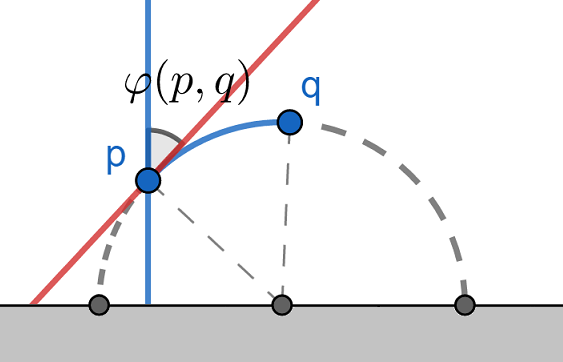
\includegraphics[width=0.5\textwidth]
  {figures/hyperbolic.png}

图:测地线$\ell(p,q)$、$\ell(p,\infty)$,以及夹角$\fai(p,q)$.
\end{figure}

事实上,由初等平面几何容易给出$\fai(p,q)$的显式表达式:
$$\fai(p,q)=\arg\left(\frac{q-\overline{p}}{q-p}\right)$$
以上出现的夹角、辐角可以取任意的分支。

\begin{notation}%Let
对于$n\geq 0$,定义
$$\Conf_n(\bbH):=\{(p_1,...,p_n)\in\bbH|
p_i\neq p_j,\,\forall i\neq j\}$$
则$\Conf_n(\bbH)$有自然的$2n$维光滑流形结构($\bbR^{2n}$的开子流形)。

%For each arrow in $\Gamma$,
对于图$\Gamma=(\Gma_0,\Gma_1,\veps)\in G_n$,
以及$e\in\Gma_1$,定义流形$\Conf_n(\bbH)$上的光滑函数$\fai_e$如下:
\begin{eqnarray*}
\fai_e:\Conf_n(\bbH)&\to&\bbR\\
(p_1,...,p_n)&\mapsto&\fai(p_{s(e)},p_{t(e)})
\end{eqnarray*}
其中特别规定$p_L=0\in\overline{\bbH}$,
以及$p_R=1\in\overline{\bbH}$
\end{notation}

粗俗地说,对于图$\Gma\in G_n$,
$\Conf_n(\bbH)$当中的一个元素$\bfp$可以视为
“将图$\Gma$嵌入双曲平面$\bbH$的一种方式”:
图$\Gma$的“一般顶点”的位置由$\bfp$给出,
“特殊顶点”$L,R$分别位于$0,1$;
图$\Gma$当中的边对应于$\bbH$中的测地线。
此时,$\fai_e$可以认为是边$e$的“倾斜角”。

\begin{definition}
对于图$\Gma\in G_n$,定义
$$
  \omg_{\Gamma}=\frac{1}{n!(2\pi)^{2n}}
  \int_{\Conf_n(\bbH)}
    \bigwedge_{i=1}^n(\td\fai_{a_i}\wedge\td\fai_{b_i})
$$
%check: it is convergent.
\end{definition}
这是$2n$-形式在$2n$-维流形上的积分。
但需要验证此积分的收敛性,这里从略。
注意积分号前的系数$\frac{1}{n!(2\pi)^{2n}}$
是精心挑选的,我们稍后给出解释。
%见Kontsevich的原始论文

现在,我们可以完整地陈述以下定理:
\begin{thm}(Kontsevich)

任意的泊松流形$(X,P)$都存在形变量子化,
并且星积可以由以下公式显式给出:%The formula
$$
  f\star g
=
  \sum_{n=0}^{\infty}
    \hbar^n
    \left(
      \sum_{\Gma\in G_n}
        \omg_{\Gma}
        B_\Gma(f,g)
    \right)
$$
%gives a deformation quantization of $P$
\end{thm}
在此述而不证。构造如此星积$\star$的动机、
想法,来自于量子场论等物理背景,我们在后文会介绍之。

\begin{example}($\omg_{\Gma}$最基本的显式计算)

我们考虑简单(但重要的)情形:$\Gma,\Gma'\in G_1$分别为如下:
$$
  \xymatrix{
    &1\ar[dl]_{a_1}  \ar[dr]^{b_1}
    &
  \\
     L
    &
    &R
  }
\quad
   \xymatrix{
    &1\ar[dl]_{b_1}  \ar[dr]^{a_1}
    &
  \\
     L
    &
    &R
  }
$$
那么有
$$\omg_\Gma=\frac{1}{2}\quad,\quad \omg_{\Gma'}=-\frac{1}{2}$$
\end{example}

\begin{proof}
我们只需要求$\omg_{\Gma}$,
而注意到$\Gma$与$\Gma'$的区别仅仅是两条边对换,
从而倾斜角$\fai_{\Gma,a_1}=\fai_{\Gma',b_1}$,
$\fai_{\Gma,b_1}=\fai_{\Gma',a_1}$,
再由外积的反对称性,容易观察出$\omg_{\Gma}=-\omg_{\Gma'}$.

现在计算$\omg_\Gma$.
此时$n=1$,$\Conf_1(\bbH)\cong H$,
对任意的$z=x+iy\in\bbH\cong\Conf_1(\bbH)$,
由初等几何容易知道
$$
  \begin{array}{ll}
    \fai_{a_1}(z)=-2\arg z\\
    \fai_{b_1}(z)=-2\arg(z-1)
  \end{array}
$$
(允许相差$2\pi$的整数倍,这无所谓)从而
$$
    \td\fai_{a_1}(z)=-2\td\arctan\left(\frac{y}{x}\right)
=-2\frac{x\td y-y\td x}{x^2+y^2}
$$
同理
$$\td\fai_{b_1}(z)=-2\frac{(x-1)\td y-y\td x}{(x-1)^2+y^2}$$
因此有
\begin{eqnarray*}
     \omg_\Gma
&=&
     \frac{1}{1!(2\pi)^{2\times1}}
     \int_{\Conf_1(\bbH)}
       \td\fai_{a_1}
       \wedge
       \td\fai_{b_1}\\
&=&
     \frac{1}{4\pi^2}
     \int_{\bbH}
       \frac{4y}
            {(x^2+y^2)\big((x-1)^2+y^2\big)}
       \td x\wedge\td y\\
&=&
     \frac{1}{\pi^2}
     \int_{0}^{\pi}
       \sin\theta
       \td\theta
     \int_0^{\infty}
       \frac{1}
            {r^2-2r\cos\theta+1}
       \td r\\
&=&
     \frac{1}{\pi^2}
     \int_{0}^{\pi}
       (\pi-\theta)
       \td\theta
=
     \frac{1}{2}
\end{eqnarray*}
\end{proof}

\begin{rem}
事实上,如果泊松张量的分量$P^{ij}$在局部上是常值的,
那么Kontsevich给出的量子化公式刚好是Moyal星积
(见例子\ref{Moyal星积-def}),
从而Kontsevich量子化$\star_K$是Moyal星积$\star_M$的推广。
回顾我们此前已经给出了Moyal星积的显式表达式
$$f\star_M g=\sum_{k=0}^{\infty}\frac{\hbar^k}{k!}
\sum_{|I|=|J|=k}P^{I,J}(\p_If)(\p_Jg)$$
\end{rem}

\begin{proof}
我们来考察$P^{ij}$为常数的情形。对于$n\geq 0$,以及$\Gamma\in G_n$,
注意到如果$\Gma$当中有箭头不指向$L$且不指向$R$,则双微分算子$B_\Gma$
当中含有对$P^ij$求导的项,因此$B_\Gma=0$,对$\star_K$没有贡献。
从而我们只需要考虑$G_n$的子集
$$\widetilde{G_n}:=\{\Gma\in G_n|t(a_i)\in\{L,R\},\forall 1\leq i\leq n\}$$
即,$\widetilde{G_n}$当中的图具有性质:每个箭头都指向$L$或者$R$;
并且容易知道$\widetilde{G_n}$当中有$2^n$个元素。
现在,
$$
  f\star_K g=
  \sum_{n=0}^{\infty}
    \hbar^n
    \sum_{\Gma\in\widetilde{G_n}}
      \omg_{\Gma}B_{\Gma}(f,g)
$$
再注意到,对于任意$\Gma,\Gma'\in\widetilde{G_n}$,都有
$$\omg_{\Gma}B_{\Gma}=\omg_{\Gma'}B_{\Gma'}$$
这是由于两个$1-$形式的外积具有反交换性,
以及泊松张量分量$P^{ij}$关于指标的反对称性。
从而我们不妨取$\widetilde{G_n}$中的代表元
$\Gma^n\in\widetilde{G_n}\subseteq G_n$,其中$\Gma^n$满足:
所有的边$a_i$都指向$L$,所有的边$b_i$都指向$R$.从而
\begin{eqnarray*}
  f\star_K g
&=&
  \sum_{n=0}^{\infty}
    \hbar^n
      2^n\omg_{\Gma^n}B_{\Gma^n}(f,g)\\
&=&
  \sum_{n=0}^{\infty}
    \hbar^n2^n
      \omg_{\Gma^n}
      (P^{a_1b_1}\cdots P^{a_nb_n})
      (\p_{a_1}\cdots\p_{a_n}f)
      (\p_{b_1}\cdots\p_{b_n}g)
\end{eqnarray*}
最后再注意到
\begin{eqnarray*}
     \omg_{\Gma^n}
&=&
     \frac{1}{n!(2\pi)^{2n}}
     \int_{\bbH^n}
       \bigwedge_{i=1}^n
         (
         \td\fai_{a_i}(z_i)\wedge
         \td\fai_{b_i}(z_i)
         )\\
&=&
     \frac{1}{n!(2\pi)^{2n}}
     \prod_{i=1}^n
       \left(
         \int_{\bbH}
           \td\fai_{a_i}(z_i)\wedge
           \td\fai_{b_i}(z_i)
       \right)\\
&=&
     \frac{(2\pi^2)^n}{n!(2\pi)^{2n}}
 =
     \frac{1}{n!2^n}
\end{eqnarray*}
因此Kontsevich量子化$\star_K$满足
\begin{eqnarray*}
  f\star_K g
&=&
  \sum_{n=0}^{\infty}
    \hbar^n2^n
      \frac{1}{n!2^n}
      (P^{a_1b_1}\cdots P^{a_nb_n})
      (\p_{a_1}\cdots\p_{a_n}f)
      (\p_{b_1}\cdots\p_{b_n}g)\\
&=&
     \sum_{n=0}^{\infty}
      \frac{\hbar^n}{n!}
      (P^{a_1b_1}\cdots P^{a_nb_n})
      (\p_{a_1}\cdots\p_{a_n}f)
      (\p_{b_1}\cdots\p_{b_n}g)\\
\end{eqnarray*}
这正是Moyal乘积的表达式。
\end{proof}

%\begin{rem}
%if $P^{ij}$ is constant, then this is Moyal product.
%(也就是说,这是Moyal pruduct 的推广)
%结合性很不显然2333333
%以后会解释这个公式的来历。物理背景+非交换技术....
%\end{rem}

%%%%现在开始正课,刚才的故事讲完了%%%

\section{量子场论背景、BV算子}
%\textbf{Some basis of QFT}
现在我们开始逐渐去理解Kontsevich的形变量子化的构造;
为此需要一些\textbf{量子场论}
(quantum field theory,简称QFT)背景知识。
\index{quantum field theory\kong 量子场论}

%a physics system always consists of
%$$\mcalS:\mcalE\to\bbR$$
%where $\mcalE$ is the space of field( of infinity dimension)

大致地说(并非严格的数学表述),一个\textbf{物理系统}
包括以下要素:\textbf{场空间}(space of fields)
$\mcalE$与\textbf{作用量}
(action functional)$\mcalS$,
\index{space of fields\kong 场空间}
\index{action functional\kong 作用量}
其中场空间$\mcalE$通常为无穷维空间,作用量
$$\mcalS:\mcalE\to \bbC$$
为场空间$\mcalE$上的函数。
%$\mcalS$ : actional functional%作用量

在经典物理中,态的演化常用变分的临界来描述态的演化:
%Classical physics:
$$\Crit(\mcalS)=\{\delta\mcalS=0\}$$
上式中的$\Crit(\mcalS)$称为$\mcalS$的critical locus,
$\delta$为某个变分导数。
\index{critical locus}

%Quantum physics:
而在量子物理中,态的演化与积分
$$\int_{\mcalE}\mcalO e^{i\mcalS/\hbar}$$
有关,其中$\mcalO$为$\mcalE$上的函数,
称之为\textbf{观测量}(observable);
\index{observable\kong 观测量}
上述积分称之为“\textbf{路径积分}”(path integral)。
\index{path integral\kong 路径积分}

不过要注意,$\mcalE$是无穷维空间,
在$\mcalE$上面积分是说不清道不明的事情;
我们至今还未完全搞明白此积分的严格定义。
我们在本讲义只谈论“数学上的事情”,
数学上暂时没说清楚的东西避而不谈。

%"path integral", $\theta$ is a function on $\mcalE$("observable").

\begin{example}作为场空间$\mcalE$的例子,
以下是近代物理中的常见对象:
$$
  \begin{tabular}{|c|c|}
  \hline
  标量场论    &  $\mcalS=$流形$X$上的全体光滑函数\\
  \hline
  规范理论    &  $\mcalS=$向量丛$E\to X$上的全体联络\\
  \hline
  $\sgm$-模型 &  $\mcalS=$流形$\sgm$与$X$之间的全体光滑映射\\
  \hline
  引力理论    &  $\mcalS=$流形$X$上的全体黎曼度量\\
  \hline
  \end{tabular}
$$
\end{example}

我们再举一些作用量$\mcalS$的例子:

\begin{example}(作用量)

(1)在标量场论$\mcalE=C^{\infty}(X)$中,
对于$X$上的光滑函数$\fai\in\mcalE$,定义
$$\mcalS[\fai]=\int_X|\nabla\fai|^2$$
称之为能量泛函。

(2)在规范理论当中,对于$A\in\mcalE$为向量丛$E\to X$上的联络,
记其曲率张量为
$$F_A:=\td A+\frac{1}{2}[A,A]$$
定义如下的\textbf{杨-米尔斯泛函}(Yang-Mills functional)
$$\YM[A]:=\int_XF_A\wedge*F_A$$

%$$\mcalE=\{\text{connections on $E\to X$}\}$$
%curvature
%is called Yang-Mills functional.
\index{Yang-Mills functional\kong 杨-米尔斯泛函}
\end{example}

%\begin{example}
%$$\mcalE= C^{\infty}(X)$$
%$$\mcalS[\fai]=\int_X|\nabla\fai|^2\quad\fai\in C^{\infty}(X)$$
%(scalar field theory)
%$$\delta\mcalS=0\Longrightarrow\Delta\fai=0$$
%\end{example}
%\begin{example}($\sigma$-module)
%$$\mcalE=map(\Sigma,X)$$
%...
%\end{example}
%\begin{example}(Gravity)
%$$\mcalE=\{\text{metrics on $X$}\}$$
%\end{example}
%以上是四种很经典的例子。
%Problem: How to construct

一个重要的问题是,如何去构造路径积分
$$\int_{\mcalE}\theta e^{i\mcalS/\hbar}$$
我们介绍\textbf{BV方法}(Batalin-Vilkovisky method),
其主要思想是用同调理论来解释测度论。

%We introduce a different method:BV method
%(Batalin-Vilkovisky)
%Philosophy: measure theory$\int_X\mapsto$ Homology theory.....
%Calculus

我们来考察有限维的情形。设$X$为$n$维紧致定向流形,
$\Omg\in\Omg_X^n$为$X$上的一个体积形式,
则$X$上的紧支光滑函数$f$关于该体积形式的积分可以视为如下:
\begin{eqnarray*}
\int_X: C^{\infty}_c(X)&\to&\bbR\\
f&\mapsto&\int_Xf\Omg
\end{eqnarray*}

%$$\int_X:\Omg_X\updot\to\bbR$$
%where $X$ is compact oriented manifold of dimension $n$,

我们考虑
$$\Omg_c(X):=\bigoplus_{p\geq 0}\Omg_c^p(X)$$
为紧支的微分形式,以及$\td:\Omg_c^p(X)\to\Omg_c^{p+1}(X)$为de Rham外微分。
众所周知,
$$H^n(\Omg_c\updot(X),\td)\cong\bbR$$
此式可以给出积分$\int_X$的同调解释:
\begin{eqnarray*}
\int_X:C_c^{\infty}(X)&\to&\bbR\\
f&\mapsto&[f\Omg]\in H^n(\Omg_c\updot(X),\td)\cong\bbR
\end{eqnarray*}

粗俗地说,我们把求$f$关于体积形式$\Omg$的积分
视为取$f\Omg$的同调类;在此意义下,de Rham复形
$(\Omg_C\updot,\td)$扮演了“测度”的角色。

%Observe:
%$$H^n_{DR}(X)=H^n(\Omg\updot,\td)\cong\bbR$$
%$$\int_X:\Omg^n\to H^n_{DR}\cong\bbR$$
%$$\alpha\mapsto[\alpha]$$
%$$\rightsquigarrow\int_X=H_{DR}^n$$
%$$(\Omg\updot(X),\td)\rightsquigarrow\text{measure}$$
%Question:how to $\int_X=H^n\quad n\to\infty$?

%%%%%%%%%%%%%%%%%%%%%%%%%%%%%%%%%%%%%%%%%%%%%%%%%%%%%%%%%
%%%%%%%%%%%%%%%%2019.3.26星期二 第五周%%%%%%%%%%%%%%%%%%%
%%%%%%%%%%%%%%%%%%%%%%%%%%%%%%%%%%%%%%%%%%%%%%%%%%%%%%%%%

%讲一些物理想法
%\textbf{Feynman Diagram}
%recall:
%$$D^n_{DR}=\int_X:\Omg\updot(X)\to\bbR$$
%what if $n\to \infty$?

在物理上我们常要面对无穷维空间,于是在此意义下,
我们需要关心$n\to\infty$时,$H^n(X)$是何物。
这是难以说清楚的,我们不妨换一个角度来看。

%Different philosophy:
%Let $\PV\updot(X):=\Gamma(X,\wedgeform{*}TX)$,
%$\Omg$ be a volume form($n$-form) on $X$,then
%$$f\mapsto\int_Xf\Omg$$
%$$\PV^k(X)\xra{\dashv\Omg}\Omg^{n-k}(X)$$
%is a 1-1 coorespondence.
%%%%缩并%%%%%%%

\begin{definition}
设$X$为$n$维紧致定向流形,$\Omg$为$X$上的一个体积形式,
则有$\Omg$诱导了多重切向量场$\PV\updot(X)$
与微分形式$\Omg_X\updot$之间的$C^{\infty}$-线性同构
\begin{eqnarray*}
\Gma_\Omg:\PV^k(X)&\to&\Omg^{n-k}_X\\
V&\mapsto& V\suobing\Omg
\end{eqnarray*}
其中$V\lrcorner\,\Omg$为$V$关于$\Omg$的缩并.
\end{definition}


在局部坐标下,若$\Omg=\td x^1\wedge\td x^2\cdots\wedge\td x^n$,
$$V=\p_{i_1}\wedge\p_{i_2}\wedge\cdots\wedge\p_{i_k}$$
为多重切向量场,其中指标$i_1<i_2<\cdots<i_k$,则容易知道
$$
  \Gma_\Omg(V)=V\suobing\Omg
= (-1)^{(i_1-1)+(i_2-1)+\cdots+(i_k-1)}
  \cdots\wedge\widehat{\td x^{i_1}}
  \wedge\cdots\wedge\widehat{\td x^{i_k}}\wedge\cdots
$$

\begin{example}
$$(\p_2\wedge\p_3)\suobing(\td x^1\wedge\td x^2\wedge\td x^3\wedge\td x^4)
=-\td x^1\wedge\td x^4$$
\end{example}
以此为例,缩并的运算规则可以理解为:
$\p_i$向右移动与$\td x^i$相遇而湮灭,
其中在$\p_i$移动的过程中穿过几个对象
($\p_j$或者$\td x^j$)就改变几次正负号
(这符合Koszul符号法则的“精神”)。

例如,如果$\Omg=e^{f(x)}\td x^1
\wedge\td x^2\wedge\td x^3\wedge\td x^4$,则
$$\Gma_\Omg(\p_2\wedge\p_3)=e^{f(x)}\td x^1\wedge\td x^4$$
再比如,对于体积形式$\Omg$本身,有
$$\Gma_\Omg^{-1}(\Omg)=1$$
也就是说$1\in\PV^0(X)$对应于$\Omg\in\Omg^n_X$.

当$V\in\PV^1(X)$为切向量场时,
$V\lrcorner\Omg=i_V(\Omg)$就是我们熟悉的内乘运算。

\begin{rem}(多重切向量场的内乘)
类似于关于切向量场$X$的内乘算子
$i_X:\Omg\updot_X\to \Omg^{\bullet-1}_X$,
我们也可以考虑多重切向量场$V\in\PV^p(X)$的内乘
$$i_V:\Omg\updot_X\to\Omg^{\bullet-p}_X$$
使得对任意$\omg\in\Omg^r_X\,(r\geq p)$,以及任意$W\in\PV^{r-p}(X)$,成立
$$\langle i_V(\omg),W\rangle=\langle\omg,V\wedge W\rangle$$
\end{rem}
特别注意,对于多重切向量场$V\in\PV\updot(X)$以及体积形式$\Omg$,
一般来说
$$V\suobing\Omg\neq i_V(\Omg)$$
它们两者之间会相差一些奇怪的正负号。
我们这里的$\PV^k(X)$与$\Omg^{n-k}_X$
的对应是通过缩并实现的,而不是内乘。

\begin{definition}(BV算子)

对于$n$维光滑定向流形$X$,
设$\Omg\in\Omg^n_X$为$X$上的一个体积形式,
定义算子$\yc_\Omg:\PV^{k}(X)\to\PV^{k-1}(X)$,使得下图交换:
$$
  \xymatrix{
     \PV^k(X)        \ar[r]^{\yc_\Omg}  \ar@{=}[d]_{\Gma_\Omg}
    &\PV^{k-1}(X)                       \ar@{=}[d]_{\Gma_\Omg}
  \\
     \Omg_X^{n-k}    \ar[r]^{\td}
    &\Omg_X^{n-k+1}
  }
$$
称$\yc_\Omg$为\textbf{BV算子}(Batalin-Vilkovisky operator)。
\index{Batalin-Vilkovisky operator\kong BV算子}
\end{definition}
%$$\PV^*(X)\leftrightarrow \Omg^{n-\bullet}(X)$$
%$$\yc\leftrightarrow \td$$
无非是将de Rham上链复形$(\Omg\updot_X,\td)$
通过体积形式同构为\textbf{上}链复形
$(\PV\updot(X),\yc_\Omg)$,其实没干什么事情。
特别注意我们规定$\PV^k(X)$的次数为$-k$,
使得$\yc_{\Omg}$是次数为$1$的微分算子(而不被看作边缘算子)。

注意到此时有上同调群的同构
$$H^n(\Omg\updot_X,\td)\cong H^0(\PV\updot(X),\yc_\Omg)$$
回顾我们对积分$\int_Xf\Omg$的同调解释,从而有
$$\int_X:f\mapsto[f]\in H^0(\PV\updot(X),\yc_\Omg)$$
也就是说我们可以把求函数$f$关于体积形式$\Omg$的积分转化成取$f$在
$(\PV\updot(X),\yc_\Omg)$的第零个同调类。这样的好处是,
容易向维数$n\to\infty$的情形推广,毕竟无论维数$n$如何升高,
我们取的总是第零个同调。

不过这样的代价是,问题转化为“如何构造无穷维空间上的BV算子”。

%this "$\yc$" is called "divergence operator w.r.t the volume form".
%when $x\in\PV^1(X)$,check: $\yc(v)=\div_{\Omg}v$.
%$$\td^2=0\Rightarrow\yc^2=0$$
%$$\PV^n\xra{\yc}\PV^{n-1}\xra{\yc}\PV^{n-2}\to\cdots$$
%$\yc$ is also called "BV operator".
%$$\int_{BV}:=H_0(\yc)$$
%good news: $0$ doesn't depend on $\dim(X)$!
%(so, we can $n\to\infty$???)
%\textbf{Difficulty}: when $n\to\infty$, we need to construct $\yc$.

\begin{rem}(广义散度)

事实上,如果$v\in\PV^1(X)$为$X$上的切向量场,则
$$\yc_\Omg(v)=\Div_\Omg(v)$$
正是我们熟悉的关于体积形式$\Omg$的散度。
\end{rem}
于是我们也俗称BV算子为多重切向量场的“广义散度”。

为了书写方便,我们引入一套高效的语言:Grassmann变量。

\begin{notation}(Grassmann变量)

对于$n$维流形$X$,以及$X$的局部坐标卡$U\subseteq X$,
我们考虑分次交换$\bbR$-代数
$$C^{\infty}(U)\ten\Free\{\theta_1,\theta_2,...,\theta_n\}\big/\sim$$
其中生成关系$\sim$为由
$\{\theta_i\theta_j+\theta_j\theta_i|1\leq i,j\leq n\}$生成的理想。
其中分次结构由
$$\deg\theta_i=-1\quad\forall 1\leq i\leq n$$
给出。
\end{notation}
容易发现,无非是将$\PV\updot(U)$当中的$\p_i$重新写为$\theta_i$,从而局部上
$$\PV\updot(U)=C^{\infty}(U)[\theta_1,...,\theta_n]$$
换句话说,$X$上的多重切向量场(局部上)
可以写为关于局部坐标$x^1,...,x^n$以及Grassmann变量的函数
$$\mu=\mu(x^1,...,x^n;\theta_1,...,\theta_n)\in\PV\updot(X)$$

{\color{blue}这里的Grassmann变量$\theta_i$是不是
Doubrovin-Zhang可积系统里面的“超变量”?
}

%\begin{example}
%Let $X$ is a manifold of finite dimension, $\dim X=n$,
%local coordinate $\{x^1,...,x^n\}$ in $\mcalU\subseteq X$,
%volume form
%$$\Omg=e^{f(x)}\td x^1\wedge\cdots\wedge\td x^n$$
%$$\Omg\updot(\mcalU):=C^{\infty}(\mcalU)[\td x^1,...,\td x^n]$$
%where $\td x^i\wedge\td x^j=-\td x^j\wedge\td x^i$.
%$\PV\updot(\mcalU):=C^{\infty}(\mcalU)[\p_1,...,\p_n]$
% where $\p^i\wedge\p^j=-\p^j\wedge\p^i$.
%\end{example}
%introduce grassman variables $\theta_1,...,\theta_n$,
%($\theta _i\cong \p_i$)
%define
%$$\PV\updot(\mcalU):=C^{\infty}(\mcalU)[\theta_1,...,\theta_n]$$
%%%%%%%非交换的微积分%%%%%%%%

\begin{definition}对于流形$X$,局部坐标下我们定义$-1$阶超导子
$$\pp{\theta_i}:\PV\updot(X)\to\PV\updot(X)$$
使得成立

  \begin{eqnarray*}
    \pp{\theta_i}f(x^1,...,x^n)=0,\qquad
    \pp{\theta_i}\theta_j=\delta^i_j
  \end{eqnarray*}

\end{definition}
$\pp{\theta_i}$服从$-1$阶超导子的超莱布尼茨法则,
即对任意$f,g\in\PV\updot(X)$为齐次元,成立
$$\pp{\theta_i}(fg)=\pfrac{f}{\theta_i}g+(-1)^{\deg f}f\pfrac{g}{\theta_i}$$

容易验证,超导子$\pp{\theta_i}$满足关系
$$\pp{\theta_i}\pp{\theta_j}=-\pp{\theta_j}\pp{\theta_i}$$
对任意$1\leq i,j\leq n$成立。特别地,$\left(\pp{\theta_i}\right)^2=0$.

\begin{prop}(BV算子的Grassmann变量表达式)

对于定向流形$X$,设体积形式
$$\Omg=e^{f(x)}\td x^1\wedge\cdots\wedge \td x^n$$
则关于$\Omg$的BV算子$\yc\Omg$在Grassmann变量的意义下具有表达式
$$\yc_{\Omg}=\pp{x^i}\pp{\theta_i}+\pfrac{f}{x^i}\pp{\theta_i}$$

%(Odd Laplacian)
%(这是BV算子的等价定义。。。)
\label{BV算子的超变量表达式-prop}
\end{prop}

\begin{proof}
直接验证之。对于任意
$$V=\mu(x^1,...,x^n)\theta_{i_1}\cdots\theta_{i_k}\in\PV^{k}(X)$$
则有
\begin{eqnarray*}
     \yc_\Omg V
&=&
     \Gma_\Omg^{-1}\circ\td\circ\Gma_\Omg(V)\\
&=&
     \Gma_\Omg^{-1}\circ\td
     \left[
       (-1)^{(i_1-1)+\cdots+(i_k-k)}\mu e^{f}
       \widehat{\td x^{i_1}}\wedge\cdots\wedge\widehat{\td x^{i_k}}
     \right]\\
&=&
     (-1)^{(i_1-1)+\cdots+(i_k-k)}
     \Gma_\Omg^{-1}
     \left[
       (\pfrac{\mu}{x^i}+\mu\pfrac{f}{x^i})e^f
       \sum_{l=1}^k
         (-1)^{i_l-l}
         \widehat{\td x^{i_1}}\wedge\cdots\wedge\td x^{i_l}
         \wedge\cdots\wedge\widehat{\td x^{i_k}}
     \right]\\
&=&
     (\pfrac{\mu}{x^i}+\mu\pfrac{f}{x^i})
     \sum_{l=1}^k
       (-1)^{l-1}
       \theta_{i_1}\cdots\widehat{\theta_{i_l}}\cdots \theta_{i_k}\\
&=&
    \left[
      \pp{x^i}\pp{\theta_i}+\pfrac{f}{x^i}\pp{\theta_i}
    \right](V)
\end{eqnarray*}
从而证毕。
\end{proof}

注意到BV算子的表达式
$$\yc_{\Omg}=\pp{x^i}\pp{\theta_i}+\pfrac{f}{x^i}\pp{\theta_i}$$
长得像二阶微分算子,甚至很像拉普拉斯算子——$\yc_\Omg$因此也被称为
\textbf{奇拉普拉斯算子}(odd Laplacian)。
\index{odd Laplacian\kong 奇拉普拉斯算子}

\begin{prop}设$X$为定向流形,
$\Omg=e^{f(x)}\td x^1\wedge\cdots\wedge\td x^n$为$X$的一个体积形式,
$\yc_\Omg$为关于$\Omg$的BV算子。定义
%Given $\yc_{\Omg}$(BV operator), we define
$$\{,\}:\PV\updot(X)\times\PV\updot(X) \to \PV\updot(X)$$
$$\{\alpha,\beta\}:=
\yc_{\Omg}(\alpha\wedge\beta)-(\yc_{\Omg}\alpha)\wedge\beta-
(-1)^{|\alpha|}\alpha\wedge\yc_{\Omg}\beta$$
即,“$\yc$成为超导子的代价”。
那么$\{,\}$不依赖于体积形式$\Omg$的选取。
%the failure of $\yc_{\Omg}$ being a derivation.
\label{另一种Schouten-Nijenhuis括号-def}
\end{prop}

\begin{proof}
直接验证即可。对任意$\alpha\in\PV^p(X)$以及$\beta\in\PV^q(X)$,成立
\begin{eqnarray*}
     \yc_\Omg(\alpha\wedge\beta)
&=&
     \pp{x^i}\pp{\theta_i}
     (\alpha\wedge\beta)
    +\pfrac{f}{x^j}\pp{\theta_j}
     (\afa\wedge\beta)\\
&=&
     \pp{x^i}
     \left(
       \pfrac{\afa}{\theta_i}
       \wedge\beta
      +(-1)^p\afa\wedge\pfrac{\beta}{\theta_i}
     \right)
    +\pfrac{f}{x^i}
     \left(
       \pfrac{\afa}{\theta_i}\wedge\beta
      +(-1)^p\afa\wedge\pfrac{\beta}{\theta_i}
     \right)\\
&=&
     \pmfrac{\afa}{x^i}{\theta_i}\wedge\beta
    +\pfrac{\afa}{\theta_i}\wedge\pfrac{\beta}{x^i}
    +(-1)^p\pfrac{\afa}{x^i}\wedge\pfrac{\beta}{\theta_i}\\
& &
    +(-1)^p\afa\wedge\pmfrac{\beta}{x^i}{\theta_i}
    +\pfrac{f}{x^i}\pfrac{\afa}{\theta_i}\wedge\beta
    +(-1)^p\pfrac{f}{x^i}\afa\wedge\pfrac{\beta}{\theta_i}\\
&=&
     (\yc_\Omg\afa)\wedge\beta
    +(-1)^p\afa\wedge(\yc_\Omg\beta)\\
& &
    +\pfrac{\afa}{\theta_i}\wedge\pfrac{\beta}{x^i}
    +(-1)^p\pfrac{\afa}{x^i}\pfrac{\beta}{\theta_i}
\end{eqnarray*}
从而得到
$$
  \{\alpha,\beta\}
=
  \pfrac{\afa}{\theta_i}\wedge\pfrac{\beta}{x^i}
 +(-1)^p\pfrac{\afa}{x^i}\wedge\pfrac{\beta}{\theta_i}
$$
从而与$\Omg$的选取无关。
\end{proof}

我们之前也见过类似的运算:Schouten-Nijenhuis括号
(见定义\ref{Schouten-Nijenhuis定义-def});
而这里的$\{,\}$是“另一个版本的Schouten-Nijenhuis括号”:

\begin{lemma}定义$\ref{另一种Schouten-Nijenhuis括号-def}$中的括号
$$\{,\}:\PV^p(X)\times\PV^q(X)\to\PV^{p+q-1}(X)$$
满足性质:对任意$\afa\in\PV^p(X),\beta\in\PV^q(X),\gamma\in\PV^r(X)$,成立:

(1)超反交换性
$$\{\afa,\beta\}=(-1)^{pq}\{\beta,\afa\}$$

(2)超莱布尼茨法则
$$\{\afa,\beta\wedge\gamma\}
=\{\afa,\beta\}\wedge\gamma
+(-1)^{(p-1)q}\beta\wedge\{\afa,\gamma\}$$

(3)若$p=q=1$,则$\{,\}$退化为切向量场李括号:
$$\{\alpha,\beta\}=[\afa,\beta]$$
\end{lemma}

注意超反交换性(1)与性质\ref{Schouten-Nijenhuis公理-prop}
的(2)在正负号上有所出入。

\begin{proof}使用表达式
$$
  \{\alpha,\beta\}
=
  \pfrac{\afa}{\theta_i}\wedge\pfrac{\beta}{x^i}
 +(-1)^p\pfrac{\afa}{x^i}\wedge\pfrac{\beta}{\theta_i}
\eqno{(*)}
$$
直接验证即可,并不困难。对于$\alpha\in\PV^p(X),\,\beta\in\PV^q(X)$
以及$\gamma\in\PV^r(X)$,有
\begin{eqnarray*}
     \{\afa,\beta\}
&=&
     \pfrac{\afa}{\theta_i}\wedge\pfrac{\beta}{x^i}
    +(-1)^p\pfrac{\afa}{x^i}\wedge\pfrac{\beta}{\theta_i}\\
&=&
     (-1)^{(p-1)q}\pfrac{\beta}{x^i}\wedge\pfrac{\afa}{\theta_i}
    +(-1)^{p+p(q-1)}
     \pfrac{\beta}{\theta_i}\wedge\pfrac{\afa}{x^i}\\
&=&
     (-1)^{pq}
     \left(
       \pfrac{\beta}{\theta_i}\wedge\pfrac{\afa}{x^i}
      +(-1)^q\pfrac{\beta}{x^i}\wedge\pfrac{\afa}{\theta_i}
     \right)\\
&=&
     (-1)^{pq}\{\beta,\alpha\}
\end{eqnarray*}
于是超反交换性成立;再看超莱布尼茨法则,
\begin{eqnarray*}
     \{\afa,\beta\wedge\gamma\}
&=&
     \pfrac{\afa}{\theta_i}\wedge
     \pp{x^i}(\beta\wedge\gamma)
    +(-1)^p\pfrac{\afa}{x^i}\wedge
     \pp{\theta_i}(\beta\wedge\gamma)\\
&=&
     \pfrac{\afa}{\theta_i}\wedge
     \left(
       \pfrac{\beta}{x^i}\wedge\gamma
      +\beta\wedge\pfrac{\gamma}{x^i}
     \right)
    +(-1)^p\pfrac{\afa}{x^i}\wedge
     \left(
       \pfrac{\beta}{\theta_i}\wedge\gamma
      +(-1)^q\beta\wedge\pfrac{\gamma}{\theta_i}
     \right)\\
&=&
     \{\alpha,\beta\}\wedge\gamma
    +(-1)^{q(p-1)}
     \beta\wedge\pfrac{\afa}{\theta_i}\wedge\pfrac{\gamma}{x^i}
    +(-1)^{pq+p+q}
     \beta\wedge\pfrac{\afa}{x^i}\wedge\pfrac{\gamma}{\theta_i}\\
&=&
     \{\alpha,\beta\}\wedge\gamma
    +(-1)^{(p-1)q}\beta\wedge\{\alpha,\gamma\}
\end{eqnarray*}
而(3)是更加容易验证的,从略。
\end{proof}
可以体会到Grassmann变量$\theta_i$以及超导子$\pp{\theta_i}$在
张量计算上的优越性:将本该必然面对的数学归纳法、
组合恒等式转化为直接的暴力计算。

{\color{gray}
事实上,我们还可以用$(*)$来暴力验证$\{,\}$的超雅可比恒等式:
$$
  (-1)^{pr}\{\{\afa,\beta\},\gamma\}
 +(-1)^{qp}\{\{\beta,\gamma\},\afa\}
 +(-1)^{rq}\{\{\gamma,\afa\},\beta\}
=0
$$
或者换句话说
$$\{\alpha,\{\beta,\gamma\}\}=(-1)^{p-1}\{\{\alpha,\beta\},\gamma\}
+(-1)^{(p-1)(q-1)}\{\beta,\{\afa,\gamma\}\}$$
(但是这个看起来不像是导子的样子)(此处待仔细验证)
}

%Check: $\{,\}$ is a Schouten-Nijenhuis bracket(up to sign).
%(independent of the choice of $f(x)$)
%In particular,$\{,\}$ is independent of choice of $\Omg$.
%\textbf{Quantization}
%$$\{,\}\xra{?}\yc_{\Omg}$$
%这个过程与量子化的过程是一样的??WTF??

\section{费曼图}
%\textbf{Feymann Diagram}
首先我们考察一个BV算子的例子:
\begin{Example}
考虑一维流形$X=\bbR$,体积形式
$$\Omg:=\frac{1}{\sqrt{2\pi}}e^{-\frac{1}{2}x^2}\td x$$
则BV算子
$$\yc_{\Omg}=\pp{x}\pp{\theta}-x\pp{\theta}$$

特别地,我们得到
$$
  \int_\bbR x^k\Omg
=
  \left\{
    \begin{array}{ll}
      0          &  x=2k+1\\
      (2k-1)!!   &  x=2k
    \end{array}
  \right.
$$
%符号可能不对,小心check
%$\PV=\bbR[x,\theta]$, and
%$$\int_{BV}:\bbR[x,\theta]\mapsto H^0(\yc_{\Omg})$$
\end{Example}

\begin{proof}
注意
$$\Omg=e^{-\frac{1}{2}(x^2-\log 2\pi)}\td x$$
从而由性质\ref{BV算子的超变量表达式-prop},直接写出
$$\yc_{\Omg}=\pp{x}\pp{\theta}-x\pp{\theta}$$

注意到积分的(上)同调解释
\begin{eqnarray*}
  \int_X:C^{\infty}&\to& H^0(\PV\updot(X),\yc_\Omg)\cong\bbR\\
  g&\mapsto& [g]
\end{eqnarray*}
而注意到对任意$x^k\theta\in \PV^1(X)$,
在$H^0(\PV\updot(X),\yc_\Omg)$当中成立
$$0=[\yc\Omg x^k\theta]=(\pp{x}\pp{\theta}-x\pp{\theta})[x^k\theta]
=k[x^{k-1}]-x^{k+1}$$
因此对任意$k\geq 0$,成立
$$[x^{k+2}]=(k+1)[x^k]$$
递推得
$$
  [x^n]=
  \left\{
    \begin{array}{ll}
      (2k-1)!![1]  & n=2k\\
      (2k)!![x]    & n=2k+1
    \end{array}
  \right.
$$
最后注意到
\begin{eqnarray*}
\int_\bbR
  \frac{1}{\sqrt{2\pi}}
  e^{-\frac{1}{2}x^2}\td x=1\qquad
\int_\bbR
  \frac{x}{\sqrt{2\pi}}
  e^{-\frac{1}{2}x^2}\td x=0
\end{eqnarray*}
从而完。
\end{proof}
%$$\int:\bbR[x]\to\bbR$$
%$$g\mapsto\int_{\bbR}g\Omg$$
%if $g=g(x)$, then $\yc_{\Omg}g=0$. Let $[g]$ be the
%$\yc_{\Omg}$- homology class,
%$$\yc_{\Omg}(x^{m-1}\Omg)
%=(m-1)x^{m-2}
%-x^m$$
%$$\Rightarrow [x^m]=(m-1)[x^{m-2}]$$
%so,
%$$
%[x^m]=
%\left\{
%  \begin{array}{cc}
%    0  &  m \text{ is odd}\\
%    (2k-1)!![1]  & m=2k
%  \end{array}
%\right.
%$$
%so,
%$$\int_{\bbR}x^{2k}\Omg=
%(2k-1)!!\int_{\bbR}\Omg=(2k-1)!!$$

\begin{lemma}条件接上,仍考虑体积形式
$$\Omg:=\frac{1}{\sqrt{2\pi}}e^{-\frac{1}{2}x^2}\td x$$
定义算子$\mcalU:\bbR[x,\theta]\to\bbR[x,\theta]$为
$$\mcalU:=
  e^{\frac{1}{2}\pp{x}\pp{x}}$$
则BV算子$\yc_\Omg$满足
$$\yc_{\Omg}=\mcalU^{-1}(-x\pp{\theta})\mcalU$$
\end{lemma}

\begin{proof}注意到众所周知的公式%use the formula
$$e^ABe^{-A}=e^{\ad_A}B$$%then
特别地,在这里%$$\yc_{\Omg}=\pp{x}\pp{\theta}-x\pp{\theta}$$
$$A=-\frac{1}{2}\pp{x}\pp{x},\qquad B=-x\pp{\theta}$$%then

注意到
\begin{eqnarray*}
[A,B]=  
     \frac{1}{2}
     [\pp{x}\pp{x},x\pp{\theta}]
=    \pp{x}\pp{\theta}
\end{eqnarray*}
进而
$$[A,[A,B]]=-\frac{1}{2}[\pp{x}\pp{x},\pp{x}\pp{\theta}]=0$$
于是
\begin{eqnarray*}
     \mcalU^{-1}(-x\pp{\theta})\mcalU
&=&
     x^ABe^{-A}
 =
     e^{\ad A}B\\
&=&
     B+[A,B]
 =
     -x\pp{\theta}+\pp{x}\pp{\theta}
 =
     \yc_\Omg
\end{eqnarray*}
从而得证。
%$$e^ABe^{-A}=\pp{x}\pp{\theta}$$
%where $[A,[A,B]]=0$.
\end{proof}

%so,
%$$\mcalU\circ\yc_{\Omg}=(-x\pp{\theta})\circ\mcalU$$
%so,
%$$\mcalU:(\bbR[x,\theta,\yc_{\Omg}])\to
%(\bbR[x,m\theta],-x\pp{\theta})$$
%is a co-chain map.
此引理表明,有如下的交换图表:
$$
  \xymatrix{
     \bbR[x,\theta] \ar[r]^{\yc_\Omg}  \ar[d]^{\mcalU}
    &\bbR[x]                           \ar[d]^{\mcalU}
  \\
     \bbR[x,\theta] \ar[r]^{-x\pp{\theta}}
    &\bbR[x]
  }
$$
以及$\mcalU$诱导上同调群的同构
$$\mcalU:H^0(\bbR[x,\theta],\yc_\Omg)
\xra{\sim}H^0(\bbR[x,\theta],-x\pp{\theta})$$

%$$H\updot(\bbR[x,\theta],-x\pp{\theta})$$
%$$\bbR[x]\theta\xra{-x\pp{\theta}}\bbR[x]$$
%$$g\mapsto -xg(0)$$
%$H^{-1}=0$,$H^0=\bbR$.
%$$\mcalU[g(x)]_{\yc_{\Omg}}=[\mcalU(g)(x)]_{-x\pp{\theta}}
%=[\mcalU(g)(0)]_{-x\pp{\theta}}
%=\mcalU(g)(0)[1]$$

\begin{prop}条件承上,则对于任意的多项式函数$g\in\bbR[x]$,成立
$$
  \int_\bbR g\Omg
=\left.
   e^{-\frac{1}{2}\pp{x}\pp{x}}
 \right|_{x=0}g
$$
\end{prop}
%我们只谈论多项式函数,是为了偷懒,
%不太想讨论收敛性(事实上解析性质很重要)。

\begin{proof}
只需要考虑$[\mcalU(g)]\in H^0(\bbR[x,\theta],-x\pp{\theta})$。
注意到对任意$k\geq 0$,
$$-x\pp{\theta}(x^k\theta)=-x^{k+1}$$
也就是说在$H^0(\bbR[x,\theta],-x\pp{\theta})$当中,
$[x^k]=0$对任意$k\geq 1$成立,从而
$$[\mcalU(g)]=\mcalU(g)(0)
=\left.
   e^{-\frac{1}{2}\pp{x}\pp{x}}
 \right|_{x=0}g
$$
从而易得。
\end{proof}
这个性质将求积分转化为求导,大大简化运算。
(与复变函数的留数定理异曲同工?)
%so,
%$$\int_{\bbR}g(x)\Omg=\mcalU(g)(0)=
%e^{\frac{1}{2}\pp{x}\pp{x}}|_{x=0}g(x)$$
%More generally, check:

更一般地,容易证明对任意$g\in\bbR[x]$
$$\int_{\bbR}g(x+a)\Omg=
\left.
  e^{\frac{1}{2}\pp{x}\pp{x}}
\right|_{x=a}g(x)$$

\begin{Example}现在我们考虑积分%Consider the integral
$$
  \int_{\bbR}
    e^{\big(-\frac{1}{2}x^2+\frac{\lmd}{3!}(x+a)^3\big)\big/\hbar}
    \frac{\td x}{\sqrt{2\pi\hbar}}
$$
其中$\lmd,a\in\bbR$,
在这里体积形式$\Omg=e^{-\frac{1}{2}x^2/\hbar}
\frac{\td x}{\sqrt{2\pi\hbar}}$.
\end{Example}

此式中的“$-\frac{1}{2}x^2$”在物理上可以认为是“自由能”,
三次项$\frac{\lmd}{3!}(x-a)^3$则为“相互作用量”。
相互作用量的存在,使得此积分发散。

处理该积分有两种常见方式:其一是将它视为复平面上的积分,
并且重新规定积分路径(这会出现Airy函数);
或者考察它的($\hbar\to 0$的)渐近展开
$$
  \sum_{n\geq 0}\frac{1}{n!}
    \int_\bbR
      \left(
        \frac{\lmd (x+a)^3}{3!\hbar}
      \right)^n
      e^{-\frac{1}{2}x^2/\hbar}
      \frac{\td x}{\sqrt{2\pi\hbar}}
$$

%this integral is not convergent.... how to deal with it?
%(1)Change the integration Contour inside $\bbC$
%%%%%%%Contour%%%%%%%
%(Airy function)
%(2)We consider only the asymptotic series

在此我们选择后者,将$e^{-\frac{1}{2}x^2\big/\hbar}$展开,
被积函数展开后的每一项
$$
  \frac{1}{n!}
    \int_\bbR
      \left(
        \frac{\lmd (x+a)^3}{3!\hbar}
      \right)^n
      e^{-\frac{1}{2}x^2/\hbar}
      \frac{\td x}{\sqrt{2\pi\hbar}}
$$
都可以使用同调的方法计算(与之前的例子完全类似):
直接套用性质\ref{BV算子的超变量表达式-prop},此时的BV算子为
$\pp{x}\pp{\theta}-\frac{x}{\hbar}\pp{\theta}$,其实不妨相差常数倍,令
$$\yc_{\Omg}:=\hbar\pp{x}\pp{\theta}-x\pp{\theta}$$
并且令
$$\mcalU_{\hbar}:=e^{\frac{\hbar}{2}\pp{x}\pp{x}}$$
则与之前完全类似,有
$$\yc_\Omg
=\mcalU_\hbar^{-1}\circ
\left(-x\pp{\theta}\right)\circ\mcalU_\hbar$$
从而易知
\begin{eqnarray*}
     \int_\bbR
       e^{\big(
            -\frac{1}{2}x^2
            +\frac{\lmd}{3!}(x+a)^3
          \big)
          \big/\hbar}
       \frac{\td x}{\sqrt{2\pi\hbar}}
&\sim&
     \sum_{m\geq 0}\frac{1}{m!}
       \int_\bbR
         \left(
           \frac{\lmd(x+a)^3}{3!\hbar}
         \right)^m
         e^{-\frac{1}{2}x^2\hbar}
       \frac{\td x}{\sqrt{2\pi\hbar}}\\
&=&
     \left.
       \sum_{m\geq 0}\frac{1}{m!}
         e^{\frac{1}{2}\hbar\pp{x}\pp{x}}
         \left(
           \frac{\lmd x^3}{3!\hbar}
         \right)^m
     \right|_{x=a}\\
&=&
     \sum_{k,m\geq 0}
       \frac{1}{k!}
       \frac{1}{m!}
       \left(
         \frac{1}{2}\hbar\p_a^2
       \right)^k
       \left(
         \frac{\lmd a^3}{3!\hbar}
       \right)^m
\end{eqnarray*}



%%%%%%%%微积分%%%%%%%%%
introduce graph with cubic vertex,

each edge: we put $\hbar\pp{a}\pp{a}$

each point: we put $\frac{\lmd a^3}{3!\hbar}$

$$\omg_{\gamma}(a)$$
by the above rule.

%%%%%%这又是什么图%%%%%%%


\begin{thm}(Feymann graph formula)

this integration is
$$
   \int_{\bbR}
     e^{(-\frac{1}{2}x^2+\frac{\lmd}{3}(x+a)^3)/\hbar}
     \frac{\td x}{\sqrt{2\pi\hbar}}
=
   \sum_{\Gamma:\text{trivalent graphs}}
     \frac{w_{\Gamma}(a)}
          {|\text{Aut}(\gamma)|}
=
   \sum
$$
\end{thm}
\begin{proof}
check.
\end{proof}

In general, consider

%%%%%%%%%%%%%%%%%%%2019.4.1 第六周周一%%%%%%%%%%%%%%%%%%%%%%%

Recall:费曼图——理解积分的渐近展开式。

Asymptotic expansion of 
$$\int_\bbR e^{(-\frac{1}{2}x^2+I(x+a))/\hbar}\frac{\td x}{\sqrt{2\pi t_0}}$$
where
$$I(x)=\sum_{n\geq 3}\frac{\lmd_n}{n!}x^n
=e^{\frac{\hbar}{2}\p_x^2}e^{I(a)/\hbar}$$

Feymann Graph formula

$$=\exp\left(\sum_{\Gamma-\text{Commu graphs}}
\frac{\omg_\Gamma(a)}{|Aut(\Gamma)|}\right)$$

Let
$$\mcalP=\frac{1}{2}\p_a^2$$
is called propagator(传播子)
$$e^{\omg(\mcalP,I)/\hbar}=e^{\hbar\mcalP}e^{I/\hbar}$$
$$\omg(\mcalP,I)=\hbar\sum_{\Gamma}\frac{\omg_\Gamma(\mcalP,I)}{|Aut(\Gamma)|}$$

$$I\mapsto\omg(\mcalP,I)$$ 


Today:
\section{传播子与重整化群流算子}

\begin{prop}
Let $\bbR\fps{,\hbar}^+=x^3\bbR\fps{x}\oplus\hbar\bbR\fps{x,\hbar}\subseteq\bbR\fps{x,\hbar}$,
(at least cubic modulo $\hbar$),then 
$$\omg(\mcalP,-):I\to\omg(\mcalP,I)$$
is a well-defined transformation on $\bbR\fps{x,\hbar}^+$.
$$\omg(\mcalP,-):\bbR\fps{x,\hbar}^+\mapsto\bbR\fps{x,\hbar}^+$$

and its inverse is $\omg(-\mcalP,-)$. 
\end{prop}

\begin{proof}
Let $I\in\bbR\fps{x,\hbar}^+$,
$$I=\sum_{k,g\geq 0}I_{k,g}\hbar^g$$
where $I_{k,g}$ has degree $k$ polynomial on $x$.

If $I_{k,g}\neq 0$, then $2g-2+k\geq 0$ 
and equality holds only if when $g=1,k=0$.
we need to prove 
$$\hbar\sum_{\Gamma}\frac{\omg_\Gamma(\mcalP,I)}{\hbar}$$
is well defined, and in $\bbR\fps{x,\hbar}^+$.

Let $\Gma$ be a connected graph,

…………
%%%%%%%2334%%%%%%%%%%%%%% 
%证了一页多。。。见手稿
\end{proof}

$$\bbR\fps{x,\hbar}^+\to \bbR\fps{x,\hbar}^+$$
$$I\mapsto\omg(\Gamma,I)$$
$$e^{\omg(\Gamma,I)/\hbar}=e^{\hbar\mcalP}e^{I/\hbar}$$
$\omg_(\Gamma,-)$ is called \textbf{renormalization group flow operator}.

For $\bbR^n$,consider 
$$\int_{\bbR^n}\prod_{i=1}^n\frac{\td x^i}{\sqrt{2\pi\hbar}}
e^{(-\frac{1}{2}Q(x)+I(x+a))/\hbar}$$

where $Q(x)=\sum Q_{ij}x^ix^j$ quadratic ,and $(Q_{ij})>0$ positive.
$$I(x)\in\bbR\fps{x^i,\hbar}^+$$
at least cubic in $x^i$ modulo $\hbar$.

the volume form 
$$e^{-\frac{1}{2\hbar}Q(x)}\prod_{i=1}^n\frac{\td x^i}{\sqrt{2\pi\hbar}}$$
$$\yc=\hbar\sum_i\pp{x^i}\pp{\theta_i}-\sum_{i,j}Q_{ij}x^i\pp{\theta_j}
=\mcalU^{-1}(-\sum_{ij}Q_{ij}x^i\pp{\theta_j})\mcalU$$
where 
$$\mcalU=e^{\frac{1}{2}\hbar Q^{ij}\pp{x^i}\pp{x^j}}$$
where $(Q^{ij})=(Q_{ij})^{-1}$. Then
$$\int_{\bbR^n}\prod_{i=1}^n\frac{\td x^i}{\sqrt{2\pi\hbar}}
e^{(-\frac{1}{2}Q(x)+I(x+a))/\hbar}
=\frac{1}{\sqrt{\det Q}}
  \left(
    e^{\frac{1}{2}\hbar Q^{ij}\pp{a^i}\pp{a^j}}e^{I(a)/\hbar}
  \right)
=
  \frac{1}{\sqrt{\det Q}}
  \exp\left(
    \sum_{\Gamma-\text{connected graph}}
      \frac{\omg_\Gamma(a)}{Aut(\Gamma)}
  \right)
$$
%%%%%%%%%%Feymann rule%%%%%%%%%%%%%%%%5

Similarly, 
$$\mcalP=\frac{1}{2}\sum_{i,j}Q^{ij}\pp{x^i}\pp{x^j}$$
$$\omg(\mcalP,-):\bbR\fps{x^i,\hbar}^+\to\bbR\fps{x^i,\hbar}^+$$
$$I\mapsto \omg(\mcalP,I)$$
$$e^{\omg(\mcalP,I)/\hbar}"="e^{\hbar\mcalP}e^{I/\hbar}$$
it is well defined, invertible...

Now, $\bbR^n$ when $n"\to"\infty$...

Quantum field theory case:

\begin{example}Scalar field theory,$\bbR^D$.
$$\mcalE=C^{\infty}(\bbR^D)$$
smooth functions ,
$$\bbR^n\rightsquigarrow\mcalE$$

$$\mcalS[phi]=\frac{1}{2}
\int_{\bbR^D}
  |\td\phi|^2
 +\frac{\lmd}{4!}
  \int_{\bbR^D}\phi^4
$$
for $\phi\in\mcalE$. we want 
$$\int_{\mcalE}e^{-\mcalS[\phi]/\hbar}[D\phi]$$
\end{example}

finite dimension ,
$$\bbR^n=map(n \text{points},\bbR)$$
so,
$$\mcalE=C^{\infty}(\bbR^D)"="\lim_{N\to\infty}C^{\infty}(N \text{points})$$
(取密密麻麻的点?格点场论)

$$i \text{index}\rightsquigarrow x\in\bbR^D$$
$$\sum_i\rightsquigarrow\int_{\bbR^D}\td x$$

free part: 
$$\frac{1}{2}\int_X|\td\phi|^2
=\frac{1}{2}\int_X\phi D\phi
$$
where $D=-\sum_i\pp{x^i}\pp{x^i}$ be laplacian:
$$D:\mcalE\to\mcalE$$

propagator                        
$$\mcalP=D^{-1}=D^{-1}_{x,y}$$
(is called Green's function integral kernel)

$$\Phi:\mcalE\to\mcalE$$
operator, has kernel $\Phi(x,y)$ if 
$$\Phi(f)(x)=\int\td y\Phi(x,y)f(y)$$

eg. $\Phi=\id\iff\Phi(x,y)=\delta(x-y)$ delta function.
$$D^{-1}\to D^{-1}(x,y)=\frac{1}{|x-y|^{D-2}}$$
singularity comes from infinite dimensional nature.
(Ultra-Violet singularity紫外发散)

%%%%%%%%%2019.4.2第六周周二%%%%%%%%%%%%%%%%%%%%
%这周要布置作业,要交的作业,不然跟不上了%

%我们要花两节课来讲一个重要概念:重整化
%量子场论的例子,与Hochschild理论的联系

\textbf{Renormalization(I)}

Last time: 
$$\int_{\bbR^n}e^{(-\frac{1}{2}\sum x^iQ^{ij}x^j+I(x+a))/\hbar}
\prod_{i=1}^n\frac{\td x^i}{\sqrt{2\pi\hbar}}$$
$$=\frac{1}{\sqrt{\det Q}}e^{\frac{1}{2}\hbar Q^{ij}\pp{a^i}\pp{a^j}}e^{I(a)/\hbar}$$
$$=\frac{1}{\sqrt{\det Q}}\exp
\left(
  \sum_{\Gamma}
   \frac{\omg_\Gamma(P,a)}{Aut\Gamma}
\right)$$


Field theory example:

$\phi^4$-theory on $\bbR^4$
$$\mcalE=C^{\infty}_c(\bbR^4)$$
$$\mcalS[\phi]=\int_{\bbR^4}\frac{1}{2}\phi D\phi+\frac{\lmd}{4!}\int_{\bbR^4}\phi^4$$
$$:=Q(\phi)+I(\phi)$$

$$\int_{\mcalE}[D\phi]e^{-\mcalS[\phi]/\hbar}
"="\frac{1}{\sqrt{\det Q}}\exp
\left(
  \sum_{\Gamma}
    \frac{\omg_{\Gamma}(\mcalP,I)}
         {|Aut(\Gamma)|}
\right)$$

Feymann rule...$G(x,y)$ satisfy 
$$D_xG(x,y)=\delta(x,y)$$
(analogue $Q_{ij}Q^{jk}=\delta^{k}_i$)
(Green's function)

where $$D=-\sum_i\pp{x^i}\pp{x^i}$$
is the Laplacian...

in $\bbR^4$,
$$G(x,y)=\frac{1}{|x-y|^2}$$

(in general on $\bbR^d$, $G(x,y)\sim\frac{1}{|x-y|^{d-2}}$ when $d\geq 3$)

Feyman graph formula:

tree level ($\hbar^0$)
%%%%cy%%%%%%

$$\mcalE=C_c^\infty(\bbR^4)$$
(这个无穷维空间是有拓扑的)(这个空间上的广义函数?)

这个例子讲完了,我们稍微再复杂一点,下面呢。。。

in general, for a tree diagram (loop = 0) 
%%%%%%%%another example%%%%%%
\textbf{HW:}
the Feymann integral is well-defined.

One loop($\hbar^1$)
%%%%%%%%loop%%%%%%%
(ill defined..)
(Ultra-Violent divergent...)
发散的原因是“两个点离得太近,能量太高”

处理这种发散,引入“重整化”

idea of renormalization:

observe: Green function $G$ is the "inverse of Laplacian".
$$D^{-1}=\int_0^\infty e^{-tD}\td t$$
$e^{-tD}$ is "Heat operator"..

$e^{-tD}$ is represented by an integral kernel 
$h_t(x,y)$ such that 
$$(e^{-tD}\phi)(x)=\int_{\bbR^d}h_t(x,y)\phi(y)\td y$$

on $\bbR^d$, 
$$h_t(x,y)=\frac{1}{(4\pi t)^{d/2}}e^{-\frac{|x-y|^2}{4t}}$$

check:
$$(\p_t+D_x)h_t(x,y)=0$$

\begin{prop}

(1) $h_t$ is smooth if $t>0$, and $h_t\to\delta(x,y)$ when $t\to 0$.

(2) semi-group prop:
$$\int_{\td y}h_{t_1}(x_1,y)h_{t_2}(y,x_2)=h_{t_1+t_2}(x,y)$$
i.e.
$$e^{-t_1 D}e^{-t_2D}=e^{-(t_1+t_2)D}$$
\end{prop}

and we have
$$G(x,y)=\int_0^\infty \td t h_t(x,y)$$

introduce cut-off paramaters
$$0<\veps<L<+\infty$$

Define 
$$P^L_{\veps}(x,y)=\int_\veps^L\td h_t(x,y)$$
is smooth(called regularized propagator).
$\veps$ is called uv(紫外) cut-off,
$L$ is  called IR(红外) cut-off.

idea: Replace the propagator $G$ by $P^L_\veps$ 
and analyze the behavior of the graph as $\veps\to 0$ and $L\to\infty$.

Eg:

%%%%%%%%cnm%%%%%%%%%%%%%

\begin{eqnarray*}
     (1)
&=&
     \lmd^2\int_{\bbR^4}
       \td x\phi^4(x)
         \int_\veps^L
           \frac{\td t_1}{(4\pi t_1)^2}
           \frac{\td t_2}{(4\pi t_2)^2}
             \int_{\bbR^4}
               e^{-\frac{|y|^2}{4t_1}-\frac{|y|^2}{4t_2}}\\
&=&
     \lmd^2\int_{\bbR^4}
       \td x\phi^4(x)
         \int_\veps^L
           \frac{\td t_1}{(4\pi t_1)^2}
           \frac{\td t_2}{(4\pi t_2)^2}
           \frac{(2\pi)^2}{(\frac{1}{2t_1}+\frac{1}{2t_2})^2}\\
&=&
     \frac{\lmd^2}{(4\pi)^2}
     \int_{\bbR^4}
       \td x\phi^4(x)
       \int_\veps^L
         \frac{\td t_1\td t_2}{(t_1+t_2)^2}\\
&=&
     -\frac{\lmd^2\log\veps}{(4\pi)^2}
     \int_{\bbR^4}\td x \phi(x)^4
     +\text{terms smooth when $\veps\to 0$}
\end{eqnarray*}
%%%%%%%%gou%%%%%%%%%%%%%%

idea: $\lmd\to\lmd(\veps)$ depend on $\veps$.
Consider add the following to $\mcalS$:
$$I^{CT}_1(\veps)=\frac{\hbar\lmd^2\log\veps}{(4\pi)^2}\int\td x\phi^4$$
(CT: counter term...用来抵消发散)

$$\mcalS\mapsto\mcalS+I^{CT}(\veps)$$
$$=\frac{1}{2}\int\phi D\phi+\frac{\lmd}{4!}\td x\phi^4+
\frac{\hbar\lmd^2\log\veps}{(4\pi)^2}\int\td x\phi^4$$

Feymann rule
%%%%%%%%量子修正%%%%%%%%%%

\begin{thm}[Physics](物理中少数几个正儿八经的定理)

there exists 
$$\lmd(\veps)=\lmd+\hbar\frac{\lmd^2\log\veps}{(4\pi)^2}+\hbar^2+\cdots$$
$$=\lmd+\sum_{g\geq 1}\hbar^gG_g(\lmd,\veps)$$
(dependents on $\lmd,\veps$, singular as $\veps\to 0$.)

such that Let 
$$I^{\veps}=\frac{\lmd(\veps)}{4!}\int_{\bbR^4}\td x\phi(x)^4$$
then
$$
  \lim_{\veps\to 0}\sum_{\Gamma}
  \frac{\omg_P(P_\veps^L,I^\veps)}
       {|Aut(\Gamma)|}
$$
exists.
\end{thm}

这个定理挺难证。。。不证了。。。

\begin{example}Quantum mechanics (QFT in dimension 1)

field:
$$\gamma:\bbR\to\text{a space}$$
$$t\mapsto \gamma(t)$$

$$\mcalS[\gma]=\frac{1}{2}\int\bbR\td t|\gma'(t)|^2$$
is called energy...

\end{example}

"Physics fact": For $x,y\in\bbR^d$,consider
$$\int_{\gma:[0,t]\to\bbR^d\atop\gma(0)=x,\quad\gma(t)=y}
[D\gma]e^{-\mcalS[\gma]/\hbar}
=h_t(x,y)$$

"the second story":first order formula,
$$\mcalS\to\mcalS[\cdots]$$

还是下一节课再讲吧。。。






